\documentclass{article}
\usepackage[utf8]{inputenc}
\usepackage[T1]{fontenc}
\usepackage{lmodern}
\usepackage{amsmath}
\usepackage{graphicx} % Required for inserting images
\usepackage{url}

\title{Retele De Calculatoare}
\author{Joanne d'Arch*}
\date{March-April 2025}

\begin{document}

\maketitle



\paragraph{Planned for Optional MAC}
\begin{itemize}
    \item NAT protocol
    \item OSPF 
    \item whatever else comes
\end{itemize}

\paragraph{Done}

\begin{itemize}
    \item Calcule
    \item Introducere Cisco Packet Tracer
    \item Switch
    \item Server
    \item Cabluri.Legaturi.Porturi.
    \item FTP service
    \item Router
    \item Mail service
    \item lab2
    \item lab3
    \item DHCP lab5
    \item Lab6 calcule + how-to
    \item Teorie
    \item FTP
    \item WiFi
\end{itemize}

% *not real name for privacy
\newpage




\tableofcontents
\newpage

\part{Teorie}
\section{LAN}
LAN = Local Area Network

Presupunem primim adresa random urmatoare:
\begin{center}
    154.187.96.227/14
\end{center}

Ce inseamna mai precis asta?

\textbf{154.187.96.227} reprezinta cei \textit{4 octecti} ai adresei IPv4.

\textbf{/14} reprezinta \textit{masca de retea} a adresei.

\subsection{Ce este masca de retea?}

Verbatem.

Astăzi vom vedea că o adresă IPv4 se poate descompune într-un sufix și un prefix. Ceea ce le desparte pe una de cealaltă este masca de rețea.

Masca de rețea reprezintă o successiune de N biți 1, care au rolul de a fixa pe poziție primii N biti ai adresei de rețea (de la stanga la dreapta), astfel obținând prefixul de rețea, care apartine retelei insasi si este fix.

Sufixul astfel delimiteaza spatiul de adrese IP care vor fi date dispozitivelor din subretea.

\subsection{Adica?}

Reprezentarea in binar a adresei noastre per byte este urmatoarea:
\begin{center}
   \begin{tabular}{|c|c|}
   \hline
        154 & 10011010 \\
    \hline
        187 & 10111011 \\
    \hline
        96  & 01100000 \\
    \hline
        227 & 11100011 \\
    \hline
    \end{tabular}
\end{center}

Insiruind vom obtine
\begin{center}
    10011010.10111011.01100000.11100011/14
\end{center}
Va urma sa fixam primii 14 biti din adresa.
Asta inseamna sa facem un AND logic pe primii 14 biti cu o insiruire de 14 biti 1.

\subsubsection{Adica.}
\begin{center}
   \begin{tabular}{|c|c|c|}
   \hline
        Original & 154.187.96.227/14 &  IPv4 address\\
    \hline
      4 octeti &  \underline{10011010.101110}11.01100000.11100011 & adresa  \\
    \hline
      Masca &  \underline{11111111.111111}00.00000000.00000000 & primii 14 biti \\
    \hline \hline
       AND & \underline{10011010.101110}00.00000000.00000000 &  Network Address\\
    \hline
        Decimal & 154.184.0.0/14 &  Network Address\\
    \hline
    \end{tabular}
\end{center}

Astfel se poate spune si ca o masca de retea notata "/14" este echivalenta cu masca de retea 255.252.0.0.
Deoarece acestea sunt valorile obtinute prin insiruirea de biti.

Acum vom nega toti bitii din masca pentru a face flip. Apoi aplicam un OR logic pentru a obtine valoarea maxima a adresei, avand prefixul fixat de masca mai devreme:


\begin{center}
   \begin{tabular}{|c|c|c|}
   \hline

      Network Address &  10011010.101110\underline{00.00000000.00000000} & adresa  \\
    \hline
      Masca negata &  00000000.000000\underline{11.11111111.11111111} & ultimii 18 biti \\
    \hline \hline
       OR & 10011010.101110\underline{11.11111111.11111111} & Broadcast Address\\
    \hline
        Decimal & 154.187.255.255/14 &  Broadcast Address\\
    \hline
    \end{tabular}
\end{center}
Astfel prefixul de retea ar fi format din primii 14 biti.

\begin{center}
    $10011010.101110$ fixati.
\end{center}

Ultimii 18 biti vor determina adresele efective ale dispozitivelor. Deci inca de pe acum stim ca adresele noastre vor arata ceva de genul:

\begin{center}
     $154.184+\{0-3\}.\{0-255\}.\{0-255\}$
\end{center}
 
\subsection{NA, BA, RA, DGW, DNS.}
Network Address, Broadcast Address, Range Address, Default Gateway, Domanin Name System.

NA = Adresa retelei, nu este asignabila unui user, este prima adresa a retelei, tocmai ce am calculat-o folosind masca de retea. 

BA = Adresa de broadcast, nu este asignabila unui user, este ultima adresa a retelei, folosita pentru a da mesaje tuturor dispozitivelor din retea.


RA = Range-ul de adrese asignabile utilizatorilor/dispozitivelor. (mai numiti si user hosts).

DGW = Entry/Exit point-ul din retea, pe aici vor trece toate pachetele care vor sa mearga in alta ramura de retea. (Ex tu cand cauti ceva pe google, se trece prin default gateway). 

DNS = Adresa serverului retelei, adica locul unde se trimit, pastreaza si retrimit pachete si/sau mesaje in retea atunci cand incercam comunicarea intre dispozitive. In exemplele din laborator, serverul va fi folosit pentru a pastra conturi si a trimite efectiv email-uri intre dispozitive.


\newpage


\section{Alte Date Misto + Elaborari}

\subsection{Paritate}
Avand in vedere cum masca este o succesiune de biti care stim ca trebuie sa aiba doar valori de 1 contigue la stanga si valori de 0 la dreapta, respectiv invers cand facem negare, se pot remarca urmatoarele 2 lucruri:

1)Network Address va fi mereu un numar par. (Dar nu neaparat cu 0 in decimal la final!!). 

Why? Deoarece mereu vom avea biti de 0 la capatul din dreapta al mastii cand facem AND logic, si asta ne garanteaza ca bitul de paritate din al 4-lea octet din NA va fi mereu 0.

2)Broadcast Address va fi mereu un numar impar. 

Why? Aceeasi logica, noi cand obtinem BA practic facem un OR logic cu masca negata, si pentru orice masca nenula vom avea bitul de paritate din ultimul octet egal cu 1, iar prin OR garanteaza imparitatea in BA.


\subsection{Default Gateway}Este mereu* prima adresa de ip asignabila din Range Address, adica prima dupa Network Address, sau NA+1. Aceasta este adresa pe care o vom da Router-ului din retea. (Deoarece router-ul leaga LAN-urile intre ele).

Daca:
\begin{center}
    NA:154.184.0.0/14
\end{center}
Vom avea:
\begin{center}
    DGW:154.184.0.1/14 
\end{center}

\subsection{Adresa DNS}
Este mereu* ultima adresa asignabila din Range Address, adica prima dinainte de Broadcast Address, sau BA-1. Aceasta este adresa pe care o vom da Serverului local fizic al retelei.

Eg. in exemplul nostru:

\begin{center}
    BA:154.187.255.255/14
\end{center}
Vom avea:
\begin{center}
    DNS:154.187.255.254/14
\end{center}


*Mereu adica prin conventie mai mereu deoarece in lumea reala mai exista exceptii la firme private. Dar asta nu este lumea reala!

\subsection{Range Address} Este intervalul de adrese asignabile din retea, acesta incepe de la Default Gateway si se termina la Domain Name System, inclusiv. In acest interval vom asigna ip-urile pentru switch-uri si user hosts.

Mai precis, limitele noastre vor fi:

1. NA+1 (DGW)

2. BA-1 (DNS)

\textbf{Exemplu aici:}
\begin{center}
    NA = 154.184.0.0/14
    
    BA = 154.187.255.255/14
    
    RA = 154.184.0.1 - 154.187.255.254

    DGW = 154.184.0.1/14

    DNS = 154.187.255.254/14
\end{center}

Numarul de adrese asignabile este practic $2^{H}-2$. 

Unde H = lungimea de biti a sufixului sau 32-lungimea mastii.

Aici 32-14 = 18.

    \[2^{18}-2 = 262.144-2 = 262.142\] 

Nr. adrese pe care le putem asigna. Quite a lot.

Aceste adrese vor fi impartite intre user hosts si alte dispozitive.




\subsection{Clase de Adrese}

Cand vorbim de adrese IPv4, luam in considerare 5 clase de IP-uri.

Adrese publice. A,B,C sunt considerate `classfull` (pline.)
Ca sa le retineti minte usor, uitati-va la cum sunt 'fixati' primii n biti din stanga 0/128/192/224/240 sau b0000/b1000/b1100/b1110/b1111
\begin{itemize}
    \item A.    0.0.0.0 - 127.255.255.255/8 (retele mari)
    \item B.    128.0.0.0 - 191.255.255.255/16 (retele medii)
    \item C.    192.0.0.0 - 223.255.255.255/24 (retele mici)
    \item D.    224.0.0.0 - 239.255.255.255/NA (Not Allocated)
    \item E 240.0.0.0 - 255.255.255.255/NA Experiment
\end{itemize}

Adrese retele private. Foarte importante!
\begin{itemize}
    \item A.    10.0.0.0/8 = 10.0.0.0 - 10.255.255.255/8
    \item B.    172.16.0.0/12 = 172.16.0.0 - 172.31.255.255/12
    \item C.    192.168.0.0/16 = 192.168.0.0 - 192.168.255.255/16 (Remember this one)
    \item 127.0.0.0/8 Reserved for loopback (nu doar 172.0.0.1)
    \item 169.254.0.0/16 Adresa sistemului de operare.(Link Local Addressing)
\end{itemize}


\newpage
\section{WAN} (Wide Area Network)

Sa zicem ca vrem sa conectam niste zone.... Bega, Bihor, Bistrita, Babadag, Bicaz, Buzau, bun. In fiecare zona vrem sa putem avea un numar exact de useri. Cum configuram retaua?
*prin conventie, vom aloca ip-uri descrescator dupa numarul de useri din fiecare ramura de retea.


Intai vom configura fiecare LAN, apoi vom lega in serie fiecare subretea, 2 cate 2.

\begin{center}
\begin{tabular}{||c| c| c|c|c||} 
\hline 
 Ramura & N Users & Nr.IP-uri necesare & $2^{n}$ maxim $\geq N$ & IP-uri alocate \\
 \hline \hline
 Bega & 4094 & $4096_{4094+2}$ & $2^{12}$ & 4096\\   
 \hline 
 Buzau & 2046 & $2048_{2046+2}$ & $2^{11}$ & 2048\\  
 \hline 
 Bihor & 1022 & $1024_{1022+2}$ & $2^{10}$ & 1024\\  
 \hline 
 Bicaz & 511 & $513_{511+2}$ & $2^{10}$& 1024\\ 
 \hline 
 Bistrita & 127 & $129_{127+2}$ & $2^{8}$& 256\\   
 \hline
 Babadag & 31 & $33_{31+2}$ & $2^{6}$ & 64\\   
\hline \hline
\end{tabular}
\end{center}
\subsection{How to think it.}
Intai luam fiecare zona drept o retea/ramura LAN.

Pentru fiecare ramura va trebuie sa alocam N+2 adrese de ip, adica range-ul de adrese utilizatori + adresa de network + adresa de broadcast.
Totodată știm că putem aloca adrese doar în puteri de 2 (din cauza a cum functioneaza masca de rețea pe biți, am văzut mai sus).

Astfel desi, de exemplu, in Bicaz avem nevoie de 511 useri, care este mai mic de $2^{9}=512$, suntem obligati sa adaugam si inca 2 adrese, pentru network si broadcast, deci 511+2=513.


513 $>$ 512, astfel mergem la urmatoarea putere de 2. $2^{10}=1024$!!! Un numar aproape dramatic care va mai frapa in viitorul apropiat, si aici e punctul de referinta de ce avem 1024 pentru Bicaz.

Chiar daca da, adaugam 1 bit intreg si dublam raza de adrese posibile doar pentru a utiliza una, suntem obligati sa o si facem. Si astfel stim ca prefixul pentru Bicaz va fi de 10 bits, deci masca va fi de 32-10=22 bits. 

\[/22 \Leftrightarrow 255.255.252.0_{Mask-Bicaz} \]

Acelasi mod de gandire se aplica si la Babadag, Bistrita.


Ce urmeaza este sa aflam NA, BA, RA pentru fiecare dintre aceste 6 ramuri de retea, cu mentiunea ca toate acestea se vor afla in spatiul adresei de la inceput 154.187.96.227/14, care are Network Address 154.184.0.0/14 .

Deci plecam de aici, dar vom schimba in calcul masca retelei /14 (255.252.0.0) cu masca primei subretele in ordine descrescatoare dupa numarul de useri, aici Bega cu /20 (255.255.240.0). 

In concluzie incepem calculul stiind NA Bega: 154.184.0.0/20
\newpage
\subsection{LAN-urile} (Local Area Network)
\subsubsection{Exemplu Bega:}


Bega, 4096 ip-uri, sufix de 12 biti. 32-12 = 20 biti $=>$ \textbf{masca de 20 biti}.
\begin{center}
    \begin{tabular}{|c|c|}
    \hline
        Bega & 154.184.0.0/20 \\
    \hline
        NA & 154.184.0.0/20  \\
            \hline
        BA & 154.184.15.255/20\\
            \hline
        RA &  154.184.0.1 - 154.184.15.254/20 \\
            \hline
    \end{tabular}
\end{center}
Cum am obtinut Broadcast Address-ul? Network Address OR masca negata.

\begin{center}
   \begin{tabular}{|c|c|c|}
   \hline
      Network Address &  10011010.10111000.0000\underline{0000.00000000} & adresa  \\
    \hline
      Masca /20 negata  &  00000000.00000000.0000\underline{1111.11111111} & ultimii 12 biti \\
    \hline \hline
       OR & 10011010.10111000.0000\underline{1111.11111111} & Broadcast Address\\
    \hline
        Decimal & 154.184.15.255/20 &  Broadcast Address\\
    \hline
    \end{tabular}
\end{center}

\subsubsection{Exemplu Buzau:}
    
Buzau, 2048 ip-uri, sufix de 11 biti. 32-11 = 21 biti $=>$ \textbf{masca de 21 biti}.

Daca Network Address-ul pentru Bega era prima adresa a retelei noastre cea mare.

Atunci Network Address-ul pentru Buzau va fi prima adresa disponibila dupa toate adresele folosite de Bega.
In alte cuvinte, prima adresa DUPA Broadcast Address-ul lui Bega. 

*si da, X.X.15.255 + 1 va da X.X.16.0 deoarece \texttt{u\_int8} overflow.

Astfel:

\begin{center}
    $$NA_{Buzau} = BA_{Bega}+1$$
\end{center}


\begin{center}
    \begin{tabular}{|c|c|}
        \hline Buzau & 154.184.15.255 + 1 /21\\
       \hline  NA & 154.184.16.0/21  \\
       \hline BA & 154.184.23.255/21\\
       \hline RA &  154.184.16.1 - 154.184.23.254/21 \\
       \hline
    \end{tabular}
\end{center}
Cum am obtinut Broadcast address-ul?

\begin{center}
   \begin{tabular}{|c|c|c|}
   \hline
      Network Address &  \underline{10011010.10111000.00010}000.00000000 & adresa  \\
    \hline
      Masca negata &  \underline{00000000.00000000.00000}111.11111111 & masca 21 biti \\
    \hline \hline
       OR & \underline{10011010.10111000.00010}111.11111111 & Broadcast Address\\
    \hline
        Decimal & 154.184.23.255/21 &  Broadcast Address\\
    \hline
    \end{tabular}
\end{center}
    $$NA_{Bihor} = BA_{Buzau}+1 \text{ and so on and so forth}$$

\subsubsection{Toate zonele:}

Celelalte adrese, pe aceleasi reguli.


\begin{center}
    \begin{tabular}{||c|c||}
    \hline \hline
        Retea & 154.184.96.227/14 \\
    \hline \hline
        NA & 154.184.0.0/14  \\
            \hline
        BA & 154.187.255.255/14\\
            \hline
        RA & 154.184.0.1/14 - 154.187.255.254/14 \\
        \hline    \hline
    \end{tabular}
\end{center}


\begin{center}
    \begin{tabular}{|c|c|}
    \hline   
        Bega & 154.184.0.0/20 (NA Retea)\\
    \hline \hline
        NA & 154.184.0.0/20  \\
            \hline
        BA & 154.184.15.255/20\\
            \hline
        RA &  154.184.0.1/20 - 154.184.15.254/20 \\
        \hline 
    \end{tabular}
\end{center}

\begin{center}
    \begin{tabular}{|c|c|}
    \hline
        Buzau & 154.184.15.255+1/21 (BA Bega+1) \\
    \hline \hline 
        NA & 154.184.16.0/21  \\
            \hline
        BA & 154.184.23.255/21\\
            \hline
        RA &  154.184.16.1/21 - 154.184.23.254/21 \\
            \hline
    \end{tabular}
\end{center}

\begin{center}
    \begin{tabular}{|c|c|}
    \hline
        Bihor & 154.184.23.255+1/22 (BA Buzau+1) \\
    \hline \hline 
        NA & 154.184.24.0/22  \\
            \hline
        BA & 154.184.27.255/22\\
            \hline
        RA &  154.184.24.1/22 - 154.184.27.254/22 \\
            \hline
    \end{tabular}
\end{center}

\begin{center}
    \begin{tabular}{|c|c|}
    \hline 
        Bicaz & 154.184.27.255+1/22 (BA Bihor+1) \\
    \hline \hline
        NA & 154.184.28.0/22  \\
            \hline
        BA & 154.184.31.255/22\\
            \hline
        RA & 154.184.28.1/22 - 154.184.31.254/22 \\
            \hline
    \end{tabular}
\end{center}




\begin{center}
    \begin{tabular}{|c|c|}
    \hline 
        Bistrita & 154.184.31.255+1/24 (BA Bicaz+1) \\
        \hline \hline
        NA & 154.184.32.0/24  \\
            \hline
        BA & 154.184.32.255/24\\
            \hline
        RA & 154.184.32.1/24 - 154.184.32.254/24 \\
            \hline
    \end{tabular}
\end{center}




\begin{center}
    \begin{tabular}{|c|c|}
    \hline
        Babadag & 154.184.32.255+1/26 (BA Bistrita+1) \\
    \hline \hline
        NA & 154.184.33.0/26  \\
            \hline
        BA & 154.184.33.63/26\\
            \hline
        RA & 154.184.33.1/26 - 154.184.33.62/26 \\
            \hline
    \end{tabular}
\end{center}




\newpage

\subsection{Inserierea LAN-urilor}

\paragraph{Ce.}
Odata ce am configurat fiecare retea LAN in parte, mai ramane doar sa le si unim, astfel obtinand un WAN (Wide Area Network).

La fel cum mai multe tari fac un continent daca sunt apropiate sau mai multi studenti fac o asociatie mișto de studenti de matematica si informatica (și ei mișto), aici mai multe LAN-uri conectate fac un WAN.

Si desigur asta se face prin legaturi, 2 cate 2, de retele mai mici, dar care impreuna pot face un tot unitar.

Si mai multe WAN-uri au facut si fac Internetul (cel mai mișto).


*Mai exista si Personal Area Network si Metropolitan Area Network dar nu ne pasa de ele aici.

\paragraph{Cum.}

Default Gateway-ul despre care am mai tot vorbit pana acum pentru fiecare LAN va fi acum folosit pentru a permite intrarea si iesirea dintr-o retea in alta, prin extensie deci transportul datelor dintr-o retea in alta prin conexiunea punctelor de legatura intre retele (Router-ele!!1!!!1!!).

Adica atunci cand vrei sa trimiti un mesaj, sa zicem, din Romania in Japonia, pachetul de date cu mesajul va iesi din DGW-ul de acasa in cel local, in cel judetean, in cel national, in cel european, apoi presupunem asiatic dintr-un router in altul si eventual ajunge la Pop Star-ul tau favorit.

De asta vom vedea la capitolul practica faptul ca fiecare router are 2 porturi importante.

Serial 0/0/0

Serial 0/0/1

Deoarece router-ul este designed** sa fie legat in serie cu router-ul altei retele in 'stanga' si iarasi cu alt router din alta retea in 'dreapta'. Gandeste-te la un linked list, un element este format din informatia propriu zisa, si 2 pointeri la alte 2 elemente din lista, practic la fel este si aici, doar ca informatia propriu-zisa reprezinta o topologie de usersi si switch-uri, iar pointerii sunt legaturi cabluri DTE (serial Data Terminal Equipment).


**Ok si asta e o minciuna, deoarece daca ati observat, pe Router ai 4 slot-uri pentru module, si ai putea sa ai 8 porturi pentru serial deodata, dar iar, asta nu e lumea reala.




\section{Switch Addresses}
 Pentru conecta utilizatorii la retea avem nevoie de switch-uri.

Este important sa tinem minte ca fiecare switch are un maxim de 26 de porturi, deci $26^{*}$ de utilizatori per switch. 

Pentru a afla de cate switch-uri avem nevoie, impartim numarul de adrese ip asignabile la 26, si luam rezultatul rotunjit superior.

*further citation needed fiindcă avem 24 porturi FastEthernet, 2 GigabitEthernet dar mai trebuie sa te legi si de router cumva.

Dar împărțirea sigur e la 26.

Eg. Bega, cu $2^{12}-2=4094$ adrese ip asignabile:
   \[\frac{4094}{26}\approx 157,46 \rightarrow 158\]


Deci vom avea 158 adrese alocate switch-urilor.
De mentionat ca adresele switch-urilor vin mereu primele in spatiul de adrese asignabile, dupa default gateway.
Astfel, adresele 2-159 vor fi doar adrese de switch-uri. Toate adresele de dupa, vor fi adrese de user hosts.

 *De mentionat iar ca adresele dau overflow la adunare, adica daca am avea sa zicem 8190 de users, si deci 315 (impartire fixa) de switch-uri pentru Bega, atunci am da overflow in al 2-lea octet. Si 315 s-ar calcula ca 256+59, adresa ajungand de forma:
 \begin{center}
 \[154.184.\underline{0.1}/20 + 300 \rightarrow  154.184.\underline{1.60}/20\]
\end{center}







\subsection{Cum calculam range de switch-uri.} 
\subsubsection{Ex. cu Bega}.

\begingroup

(1)Pornim de la Network Address, nu este asignabila. 154.184.0.0/20

(2)Apoi urmeaza Default Gateway, asignabila dar folosita la altceva, 154.184.0.1/20

(3)Apoi este prima adresa asignabila nefolosita, 154.184.0.2/20. Bun.



Luam adresa de la Default Gateway, si adaugam numarul de switch-uri.


\begin{center}
    154.184.0.1/20 + 158 =  154.184.0.159/20
\end{center}

In final, range-ul de adrese ip pentru switch-uri va fi:

 \begin{center}
  154.184.0.2/20 - 154.184.0.159/20
\end{center}
Abia 154.184.0.160/20 va fi primul user host din Bega.

\subsubsection{Ex. cu Buzau}
Network Address-ul pentru Buzau este 154.184.16.0/21, deci DGW este 154.184.16.1/21.

Avem 2046 ip-uri asignabile si impartim la 26. Luam rezultatul si rotunjim superior.

\[\frac{2046}{26} \approx 78{,}69 \rightarrow 79 \]

Adresa de DGW este 154.184.16.1/21, astfel:

154.184.16.1+1/21     va fi primul switch $\rightarrow$ 154.184.16.2/21.

154.184.16.1+79/21 va fi ultimul switch $\rightarrow$ 154.184.16.80/21.

Intervalul de switch-uri pentru Buzau va fi:
\begin{center}
    154.184.16.2/21 -- 154.184.16.80/21
\end{center}


\subsection{Concluzie Switch-uri.}

\begin{center}
    \begin{tabular}{||c|c|c|c|c|}
    \hline \hline
       Subretea & NrUsers & IP-uri asignabile & Numar Switch-uri & Interval Switch-uri \\
    \hline \hline
        Bega & 4094 & 4094 & $4094/26 \rightarrow 158$ & 154.184.0.2/20 -- 154.184.0.159/20\\
        \hline
        Buzau & 2046 & 2046 & $2046/26 \rightarrow 79$ & 154.184.16.2/21 -- 154.184.16.80/21\\
        \hline
        Bihor & 1022 & 1022 & $1022/26 \rightarrow 40$ & 154.184.24.2/22 -- 154.184.24.41/22\\
        \hline
        Bicaz & 511 & 1022 & $1022/26 \rightarrow 40$ & 154.184.28.2/22 -- 154.184.28.41/22\\
        \hline
        Bistrita & 127 & 254 & $254/26 \rightarrow 10$ & 154.184.32.2/24 -- 154.184.32.11/24 \\
        \hline
        Babadag & 31 & 62 & $62/26 \rightarrow 3$ & 154.184.33.2/26 -- 154.184.33.4/26\\
        \hline
    \end{tabular}
\end{center}

\section{Legare Retele}
\subsection{Teorie}

Pentru a lega ramurile de retea intre ele, ne folosim de routere, pe care le conectam folosind porturile Serial 0/0/0 respectiv Serial 0/0/1.

Pentru aceste porturi vom pune adrese IP putin mai speciale, in sensul ca cele 2 routere vor forma o retea de sine statatoare cu adrese de sine statatoare pe care le folosesc doar aici pentru a se recunoaste una pe cealalta `de la departare` pe interfata Serial. 

Aceste adrese IP 'mai speciale' sunt folosite doar pentru a permite comunicarea unui router cu celalalt, dar nu are legatura cu adresa IP din reteaua LAN a routerului din topologia locala, care va fi fi pe interfata gigabitethernet 0/\{1-24\}.

Asta inseamna ca vom avea si cate o mini-retea cu 2 echipamente, care va contine asadar un total de 4 adrese IP ($2+2 \leq 2^{2}$), si deci o masca de 30bit. Asta per fiecare pereche de routere in serie!
\newpage

\subsection{Legaturile}
De menționat că aici ordinea contează, (pentru domnul profesor), în sensul ca legaturile în serie vor fi făcute în ordinea in care au fost date rețelele, adica aici: Bega, Bihor, Bistrita, Babadag, Bicaz, Buzau. 

\begin{center}
    \begin{tabular}{|c|c|}
    \hline
        R-Bega - R-Bihor & 154.184.33.63+1/26 (BA Babadag+1) \\
    \hline \hline
        NA &  154.184.33.64/30 \\
            \hline
        BA & 154.184.33.67/30\\
            \hline
        RA & 154.184.33.65/30 - 154.184.33.66/30 \\
            \hline
    \end{tabular}
\end{center}

\begin{center}
    \begin{tabular}{|c|c|}
    \hline
        R-Bihor - R-Bistrita& 154.184.33.67+1/30 (BA anterior +1) \\
    \hline \hline
        NA &  154.184.33.68/30 \\
            \hline
        BA & 154.184.33.71/30\\
            \hline
        RA & 154.184.33.69/30 - 154.184.33.70/30 \\
            \hline
    \end{tabular}
\end{center}


\begin{center}
    \begin{tabular}{|c|c|}
    \hline
        R-Bistrita - R-Babadag &154.184.33.71+1/30\\
    \hline \hline
        NA &  154.184.33.72/30 \\
            \hline
        BA & 154.184.33.75/30\\
            \hline
        RA & 154.184.33.73/30 - 154.184.33.74/30 \\
            \hline
    \end{tabular}
\end{center}


\begin{center}
    \begin{tabular}{|c|c|}
    \hline
        R-Babadag - R-Bicaz& 154.184.33.75+1/30\\
    \hline \hline
        NA &  154.184.33.76/30 \\
            \hline
        BA & 154.184.33.79/30\\
            \hline
        RA & 154.184.33.77/30 - 154.184.33.78/30 \\
            \hline
    \end{tabular}
\end{center}


\begin{center}
    \begin{tabular}{|c|c|}
    \hline
        R-Bicaz - R-Buzau & 154.184.33.79+1/30 \\
    \hline \hline
        NA &  154.184.33.80/30 \\
            \hline
        BA & 154.184.33.83/30\\
            \hline
        RA & 154.184.33.81/30 - 154.184.33.82/30 \\
            \hline
    \end{tabular}
\end{center}



\newpage
\part{Practica}


\section{Introducere Cisco Packet Tracer}
\subsection{IDE}
Aplicatia folosita pe de-a lungul laboratorului se intituleaza Cisco Packet Tracer. Este o aplicatie relativ simpla la care veti vedea imediat ce ar trebui sa schimbati in functie de gusturi.

\url{https://www.netacad.com/resources/lab-downloads?courseLang=en-US}

Totodata indiferent cat de mult va place sau nu, pentru a avea success la laborator, este cam mandatoriu sa exersati si in timpul liber cu aplicatia, sa refaceti laboratoarele de la facultate pe baza notitelor luate, si sa rescrieti comenzi in terminal pana cand le memorati, dar de preferat si invetati.

Ce urmeaza in partea de practica este sa facem calcule relativ foarte simple, sa adaugam echipamente, sa le configuram, sa le conectam, si sa simulam o retea.

\subsection{Lucruri de Baza.}
\paragraph{Layout}
In stanga-jos aveti un 2-step menu din care veti scoate toate echipamentele pe care le veti configura in Cisco Packet Tracer. Unde gasiti fiecare echipament relevant in parte este acoperit in sectiunea "Introducere Echipament".

Utilizarea se rezuma la :
\begin{itemize}
    \item[1.] Alegere sectiune (Stanga sus)
    \item[2.] Alegere subsectiune (Stanga jos)
    \item[3.] Alegere echipament.(Dreapta)
\end{itemize}

\begin{center}
    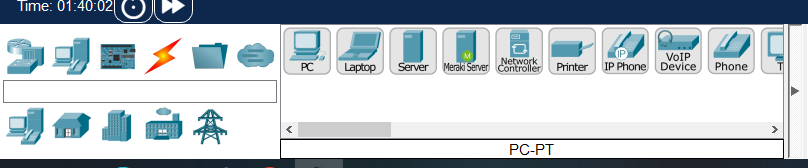
\includegraphics[width=1\linewidth]{Screenshot 2025-04-05 185830.png}
\end{center}

Daca nu folositi alte aplicatii si-sau considerati ca ecranul e prea mic per total, faceti full-screen.


    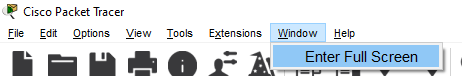
\includegraphics[width=0.5\linewidth]{Screenshot 2025-04-05 190820.png}


\paragraph{Optiuni}
In principiu o recomandare personala mai este sa mergeti la taburile din stanga-sus si sa va mariti font-ul la...mai tot. 

Si totodata puteti face sa va apara mereu port-urile folosite la capetele cablurilor.


Options $\rightarrow$ Preferences.
\begin{center}
    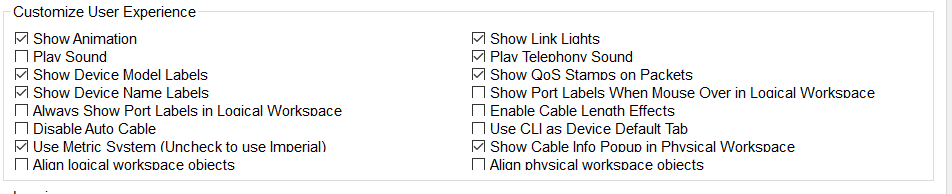
\includegraphics[width=0.75\linewidth]{Screenshot 2025-04-05 190947.png}
\end{center}

Optiuni care pot fi utile sunt, si chiar va sugerez sa va jucati cu ele:

\begin{itemize}
 \item   Show Animation (Daca folositi des Simularile din dreapta ecranului)
 \item   Show Device Model Labels
 \item   Show Device Model Names
 \item   Always Show Port Labels in Logical Workspace
 \item   Show Port Labels When Mouse Over Logical Workspace
 \item   Align Logical Workspace Objects (pune 3 note pe ecran si misca-le)
\end{itemize}

\paragraph{Zoom}
Apoi 1000$\%$ veti simti nevoia sa va mariti fontul. 



\begin{center}
    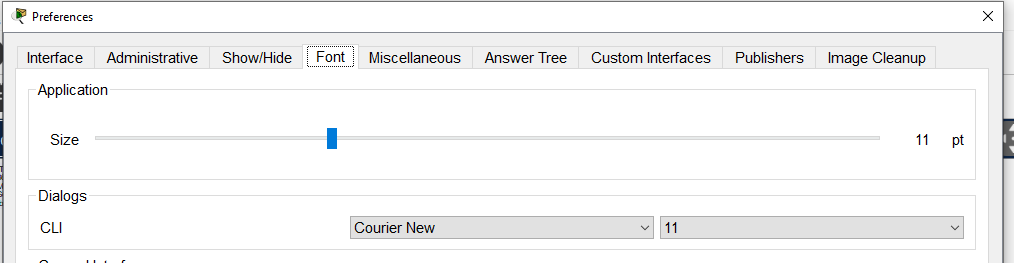
\includegraphics[width=1\linewidth]{Screenshot 2025-04-05 192617.png}
\end{center}




\paragraph{Simulari}

Daca vrei sa vezi in timp "mai" real cum comunica (sau nu) echipamentele intre ele, atunci activati tab-ul de Simulation, scrieti o comanda de CMD la un PC, precum ping, comanda va fi captata si va astepta sa activati simularea.

\begin{center}
    
\includegraphics[width=0.75\linewidth]{simulari.png}
\end{center}

\paragraph{Scenarios}

Ideea este buna dar nu le vom folosi noi, mai mult obfuscheaza echipamentele. Off with its head. Apasa butonul indicat.

\begin{center}
    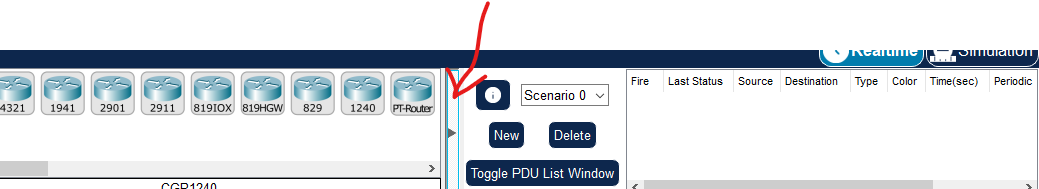
\includegraphics[width=1\linewidth]{Ascunde Scenarii.png}
\end{center}



    
\subsection{Comenzi}
Poza de jos arata Toolbar-ul Principal si Secundar (cum le numeste CPT). Aceste toolbar-uri nu sunt foarte utile deaorece comenzile se pot folosi si din mouse / tastatura.

Ca sa o ascundem: Sus $\rightarrow$ View $\rightarrow$ Toolbars

\begin{center}
    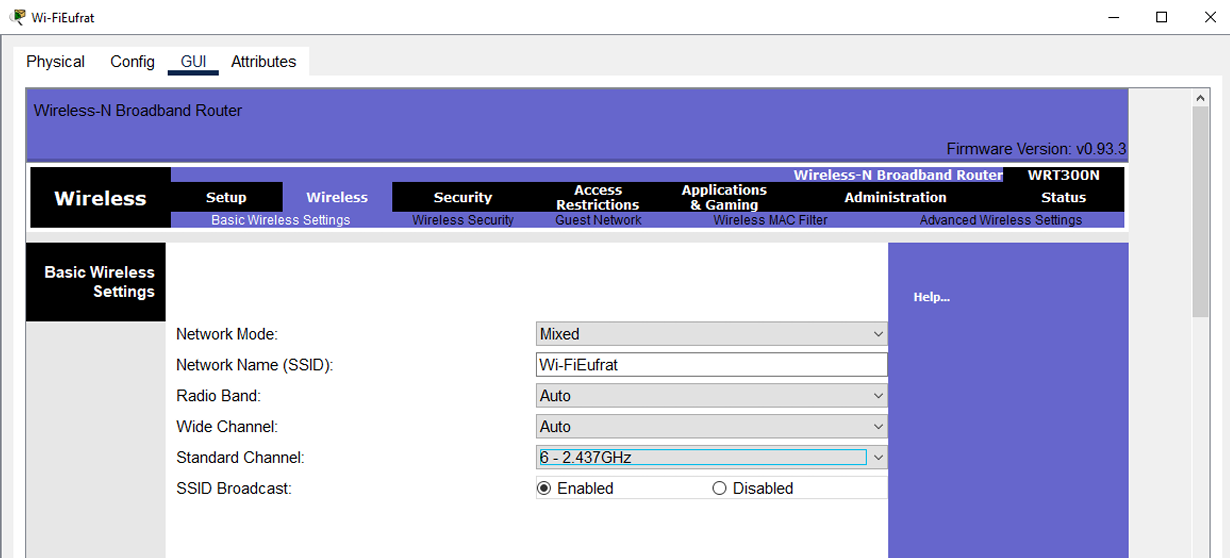
\includegraphics[width=0.75\linewidth]{BasicWirelessSettings.png}
\end{center}

Ce ne intereseaza mai mult:

\begin{itemize}
    \item Zoom in/out (Ctrl + Mouse Wheel)
    \item Delete mode (Del) - Urmatorul echipament pe care dam click va declansa un prompt daca vrem sa il stergem din topologie
    \item[!!] Note mode(N) - La urmatorul click pe mouse vom lasa pe ecran o notita ca un textbox. Este ceruta la examen.

        
    \textbf{Ceva foarte important}. In acele notite putem scrie cod LaTeX. Ce ne intereseaza este comanda \textbf{\&le;} care va aparea in acel note ca semnul de $\leq$.
    
    \item Inspect (I) - La urmatorul click pe echipament putem forta CPT sa ne arate datele de configurare setate.
    \item Cancel (Esc) - Iese din cele 3 moduri de mai sus.
\end{itemize}





\section{Introducere Echipament}
Toate echipamentele se gasesc in stanga jos pe Cisco Packet Tracer, si se pun in spatiul de munca prin Drag\&Drop sau simplu click. 

Mai mereu redenumim echipamentele cand lucram cu ele. Si deoarece noi simulan hardware fizic, pentru a le schimba componentele (Modulele care contin porturile), le vom si opri fizic din butonul de `Power Off` de pe laterala/spate! (Tab Physical)



\subsection{End User PC (Host)}
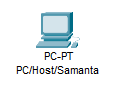
\includegraphics[width=0.2\linewidth]{PC.png}

Un Host PC care reprezinta un utilizator, pentru acesta nu avem nevoie decat sa il redenumim pentru topologie, si sa ii configuram adresa de ip si datele pentru email.

\paragraph{Locatie}:
(Stanga Jos) $\rightarrow$ End Devices $\rightarrow$ End Devices $\rightarrow$ PC (PC-PT)

\paragraph{Placa de Retea}:
Click PC $\rightarrow$ Physical $\rightarrow$Power Off$\rightarrow$ Drag \& Drop luam placa de retea $\rightarrow$ Modules $\rightarrow$ luam PT-HOST-NM-1CGE $\rightarrow$ punem in slot $\rightarrow$ Power On.

De acum mereu vom conecta PC-urile cu cabluri de tip Copper Straight-Through pe interfata de Gigabitethernet.



\paragraph{IP Configuration}:
(Click stanga PC) $\rightarrow$ Desktop $\rightarrow$ IP Configuration

\paragraph{Email}:
(Click stanga PC) $\rightarrow$ Desktop $\rightarrow$ Email



\subsection{Switch}
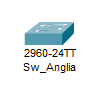
\includegraphics[width=0.25\linewidth]{Switch.png}


Switch-ul este cel ce ne permite sa legam mai multe echipamente intre ele. Are 26 de porturi, pentru toate vom folosi Copper Straight Through.

\paragraph{Locatie}:
(Stanga Jos) $\rightarrow$ Network Devices $\rightarrow$ Switches$\rightarrow$  2960



Nu are module sau alte chestii, dar nici GUI deci mereu il vom configura prin laptopul SERVICE. 

Switch-urile vor avea adrese de ip asignate ca valoare dupa adresa de ip a default-gateway-ului.

Totusi Cisco Packet Tracer a pus si un tab Config care este un fals-GUI, si mereu cand faci ceva pe el, in textbox-ul de dedesubt vor aparea comenzile ECHIVALENTE de commandline, pe care le invatam noi la laborator.

Deci este ceva util ca sa inveti comenzile la nivel atomic, dar este foarte risky la examen sa te bazezi doar pe asta.



Si de mentionat, din pagina de cod de mai tarziu, pentru ca un Switch ca functioneze (sa transmita pachete),DAR FARA securitate de vreun fel sau ssh, sunt practic necesare doar comenzile:



\begin{verbatim}
Sw_*(config)#ip domain name info.ro
Sw_*(config)#ip default gateway A.B.C.D(ip-address) 
Sw_*(config)#interface vlan 1
Sw_*(config-if)#ip address A.B.C.D(ip-address) A.B.C.D(mask)
Sw_*(config-if)#no shutdown
Sw_*(config-if)#exit
Sw_*(config)#(salvam config)
\end{verbatim}


\subsection{Router}

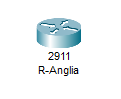
\includegraphics[width=0.25\linewidth]{Router.png}



Routerul permite comunicarea intre 2 retele LAN, si are rolul de a fi Default-Gateway-ul retelei. Deci el va avea mereu adresa IP chiar adresa de DGW, si se va lega de DGW-urile adiacente cu serial DTE. Eg comenzi de baza din lab4:
\begin{verbatim}
R-Anglia(condif-if)#ip address 192.168.50.33 255.255.255.224
R-Anglia(config)#ip route 209.100.100.160 255.255.255.224 10.10.10.10
\end{verbatim}

\paragraph{Locatie}:
(Stanga Jos) $\rightarrow$ Network Devices $\rightarrow$ Routers $\rightarrow$  2911

Copper Straight Through $\rightarrow$ Gigabitethernet 0/0 ( 0/1, 0/2).


\paragraph{Placa de Retea}:
Click Router $\rightarrow$ Physical $\rightarrow$Power Off$\rightarrow$ Drag \& Drop luam placa de retea $\rightarrow$ Modules $\rightarrow$ luam HWIC-2T $\rightarrow$ punem in al 4-lea slot, in dreapta sus langa sursa $\rightarrow$ Power On.



\subsection{Server}

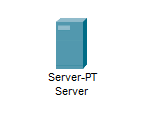
\includegraphics[width=0.25\linewidth]{Server.png}

Serverul este mai important, in sensul ca acesta ne permite accesul la numeroase servicii precum \underline{email}, syslog, DNS,FTP,etc. Pe el il conectam doar cu fir Copper Straight Through pe port Gigabitethernet 0/0.

\paragraph{Locatie Server}:

(Stanga Jos) $\rightarrow$ End Devices $\rightarrow$ End Devices $\rightarrow$ Server$\rightarrow$ Drag\&Drop$\rightarrow$Spatiu de lucru$\rightarrow$Schimbam numele.

\paragraph{Placa de Retea}:

Left Click Server $\rightarrow$ Physical $\rightarrow$ Click Power Off button $\rightarrow$ Luam placa ce era deja sus$\rightarrow$Drag\&Drop$\rightarrow$Drop at Modules $\rightarrow$Take PT-HOST-NM-1CGE$\rightarrow$ punem in slot-ul de sus.$\rightarrow$Turn On button


\paragraph{IP Configuration}:
(Click stanga Server) $\rightarrow$ Desktop $\rightarrow$ IP Configuration

\paragraph{Email}:
(Click stanga Server) $\rightarrow$ Desktop $\rightarrow$ Email
\newpage
\paragraph{Services}:
(Click stanga Server) $\rightarrow$ Services $\rightarrow$ Modules (stanga)


\begin{itemize}
    \item HTTP
        \begin{itemize}
            \item  HTTP $\rightarrow$ (BIFAT OFF)
            \item  HTTPS $\rightarrow$ (BIFAT ON)
        \end{itemize}
    \item DNS
        \begin{itemize}
            \item DNS Service $\rightarrow$ (BIFAT ON)
            \item Name $\rightarrow$ info.ro
            \item Address $\rightarrow$ Adresa DNS
            \item Type $\rightarrow$ A record
            \item Add
        \end{itemize}
    \item Email
        \begin{itemize}
            \item Domain Name $\rightarrow$ info.ro
            \item Set
            \item User $\rightarrow$ `Nume user`
            \item Password $\rightarrow$ 123456
            \item Press + button. Adaugam fiecare utilizator (adica user PC), server inclusiv.
        \end{itemize}
    \item Syslog
        \begin{itemize}
            \item Service $\rightarrow$ (BIFAT ON)
            \item aici o sa ne vedem inregistrarile samd.
            \item tine minte 3 cuvinte: Authentification Acreditation Accounting
        \end{itemize}
    \item FTP
        \begin{itemize}
            \item Service $\rightarrow$ (BIFAT ON)
            \item Username $\rightarrow$ "Nume Pc User"
            \item Password $\rightarrow$ 123456
            \item Write Read Delete Rename List Rights
            \item Add (Facem cont pentru toti userii, adica fiecare PC)
        \end{itemize}
    \item DHCP (NOT FINISHED)
        \begin{itemize}
            \item Interface $\rightarrow$ Service On
        \end{itemize}
\end{itemize}




\newpage

\subsection{Wi-Fi Router}
(Termenii "Wi-Fi Router" si "R-WiFi" sunt echivalenti in aceasta sectiune)

(Si exemplul este bazat pe laboratorul 5, cu LAN-ul Eufrat.)

Prin Wi-Fi Router putem configura conexiune wireless la internet si totodata putem permite alte dispozitive altele decat pc-uri sa se conecteze la retea, de mai oriunde. Misto.

De mentionat si faptul ca un Router Wi-Fi este tot un router, adica actioneaza drept un DGW pe LAN-ul său local si privat (192.168.X.X/24, remember adresa privata tip C)

MEREU va fi deja configurat prin default cu adresa 192.168.0.1

Cum implica acel "0.1", el reprezinta gateway-ul unui LAN propriu-zis cu adresa 192.168.X.Y/24. Sau o sa elaboram imediat... chiar mai multe sub-retele egale ca marime. 

Vom da pentru prima data un IP Laptop-ului SERVICE, deoarece Wi-Fi Router-ul NU mai are port de cablu consola, astfel singura cale de a ne conecta la el fizic pentru a-l configura este prin internet. Trebuie astfel sa dam o adresa asignabila pe care R-WiFi ar considera-o `in retea cu el` ca sa putem fi identificati de el pe internet. Adica \underline{orice adresa intre 192.168.0.2/24 - 192.168.0.254/24 inclusiv}.

Apoi vom "merge pe internet", vom cauta adresa pe care o are R-WiFi, ii vom schimba atat adresa de retea, cat si pe cea statica (elaboram mai tarziu), si vom configura serviciul de DHCP pentru a putea asigna dinamic IP-uri pentru dispozitive, in cauza niste Laptop-uri NOI pe care le vom aduce in topologie doar pentru a demonstra ca DHCP-ul si Wi-Fi-ul functioneaza.


\begin{center}
    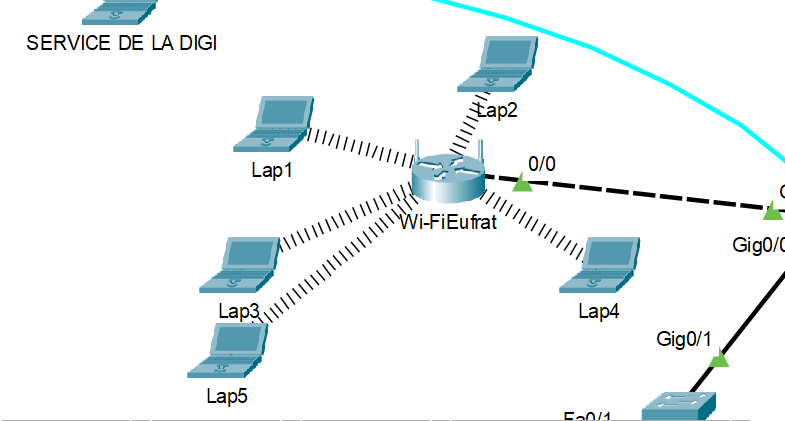
\includegraphics[width=0.5\linewidth]{Wi-FiEufrat.png}
\end{center}



\paragraph{Locatie Wi-Fi}:

(Stanga Jos) $\rightarrow$ Network Devices $\rightarrow$ Wireless Devices $\rightarrow$ WRT300N

$\rightarrow$ Drag\&Drop$\rightarrow$Spatiu de lucru$\rightarrow$Schimbam numele.
\paragraph{Config}

$\rightarrow$
\begin{itemize}

    \item[$\rightarrow$]Copper Straight-Through $\rightarrow$ SERVICE,port Fa0$\rightarrow$RWi-Fi, Ethernet 1

    \item[$\rightarrow$]Laptop SERVICE $\rightarrow$ Desktop $\rightarrow$ IP Config
    
    \item IPv4 Address $\rightarrow$ 192.168.0.X 
    
    $X \in \{2,254\}$

    \item Subnet Mask $\rightarrow$ 255.255.255.0
    
    \item[$\rightarrow$] SERVICE $\rightarrow$ Desktop $\rightarrow$ Web Browser

    \item[$\rightarrow$] Cautam url $\rightarrow$ 192.168.0.1 $\rightarrow$ GO $\rightarrow$ Authorization 
    
    \item User Name:$\rightarrow$ admin
    \item Password: $\rightarrow$ admin
    \item Ok $\rightarrow$ va aparea un meniu mare daca avem ip-ul corect.
    \begin{center}
            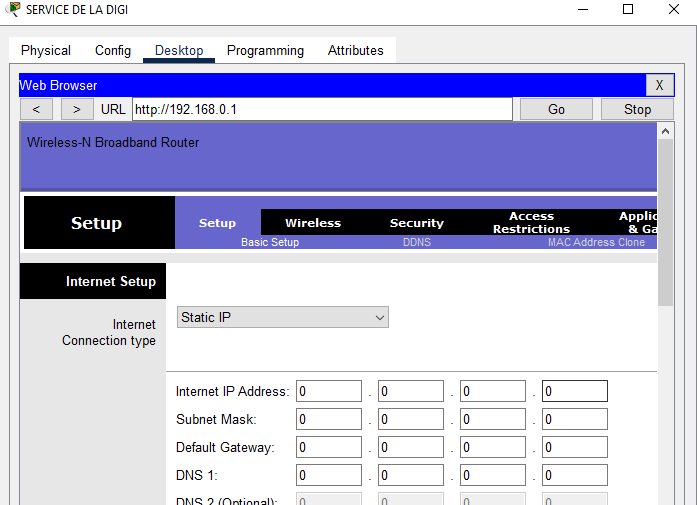
\includegraphics[width=0.75\linewidth]{Wi-FiStaticIp.png}
            
            Setup $\rightarrow$ Internet Setup $\rightarrow$ Internet Connection Type $\rightarrow$ Static IP
    \end{center}
\end{itemize}


Aici va trebui sa diferentiem dintre cele 2 ip-uri pe care le are RWi-Fi. IP-ul Static si IP-ul de retea.

IP-ul static este cel pe care il vom folosi sa conectam RWi-Fi-ul de restul topologiei prin celelalte Router-e.

IP-ul de retea este cel pe care il foloseste RWi-Fi ca default gateway pentru subreteaua de Wi-Fi locala si privata.

In meniul din poza vom pune datele pentru IP-ul static, care este acel IP din subreteaua cu 2 adrese asignabile din 4 totale, adica subreteaua de legatura cu alt router, aici R-Eufrat.*(De mentionat ca aici adresele sunt foarte mici fiindca asa a dat proful, si asta ca sa se vada distinctia cine e adresa statica si cine nu).

\paragraph{Input Static}
Continuand din meniul acela gol:

\begin{itemize}
    \item Internet IP Address $\rightarrow$ Adresa 
 cu care vom fi recunoscuti de celalalt Router( sa zicem 10.10.10.2)
    \item Subnet Mask $\rightarrow$ 255.255.255.252 (mereu)
    \item Default Gateway $\rightarrow$ 10.10.10.1 (cea mai mica dintre cele 2 adrese, adesea a celuilalt Router in subretea)
    \item DNS $\rightarrow$ ce server avem noi (sa zicem 192.168.100.110)
\end{itemize}

\paragraph{Input Network}

\begin{center}
    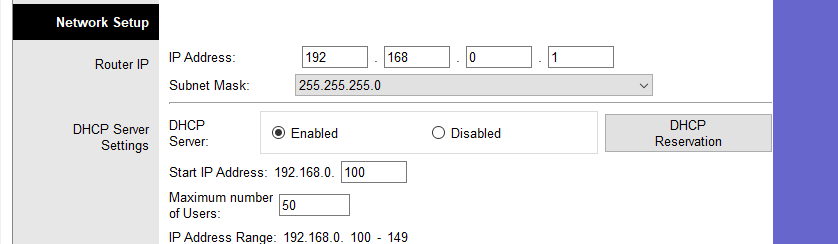
\includegraphics[width=0.75\linewidth]{Wi-Fi Network.png}
\end{center}


Acum urmeaza sa configuram intreaga retea de Wi-Fi, pentru a face asta, trebuie sa schimbam adresa si setarile de internet ale router-ului de Wi-Fi. (Ele deja exista prin default, dar noi le reconfiguram)

Deoarece reteaua de Wi-Fi este cam prin definitie o retea privata, observam urmatoarele particularitati.

\begin{itemize}
    \item[1] Adresa va fi mereu de forma 192.168.X.Y, adica vom avea o adrese din clasa C (adrese private).
    \item[2] Masca va fi cel putin /24, deoarece RWi-Fi este limitat fizic la cate dispozitive poate organiza/sustine.
    \item[3] Wi-Fi-ul este limitat la a avea 252 de useri deodata, deoarece prin masca, am putea avea maxim $2^8$ ip-uri, dintre care nu luam in considerare 3 adrese, NA,BA si DGW (RWi-Fi este deja DGW).
    \item[4] Adresa de DGW pe reteaua de Wi-Fi, adica adresa prin are identificam dispozitivil prin browser-ul web, initial era 192.168.0.1, daca schimbam adresa de DGW, va trebui sa schimbam si adresa IP din laptopul service deoarece vom pierde conexiunea.
\end{itemize}

\paragraph{Deci ce punem noi in campurile acelea?}

Network Setup $\rightarrow$ Router IP $\rightarrow$ IP Address $\rightarrow$ 192.168.X.Y

Pe o subretea de Wi-Fi putem avea un maxim de 252 de useri deodata, deci noi putem sa alocam IP-uri sub orice putere de 2 mai mica decat $2^8$. Alocarea intre puteri de 2 o facem exact ca la pasul 2 din teorie.

Dar deoarece suntem pe o adresa privata, inseamna ca avem libertate cu ce NetworkAddress ne alegem in subreteaua Wi-Fi. Astfel in al 3-lea octet putem sa punem orice numar, dar recomandarea este sa nu punem un numar mic \{0-10\} deoarece ar fi usor de ghicit pentru cineva din exterior.

O conventie este ca peste adresa de DGW initiala default a retelei Wi-Fi mari, 192.168.0.1/16, sa adaugam un multiplu al puterii de 2 din bloc-ul nostru de adrese (64,128,192) etc, si astfel adresele vor fi alocate pe blocuri de 64 de adrese (sublanuri). Noi putem alege pe oricare dintre acele blocuri, dar la lab se foloseste al 4-lea bloc. Adica daca avem 64 de adrese pe wi-fi, nu vom lua pe primele 64 (de la adresa 0-63), nici pe celelalte 64 (de la adresa 64-127) sau urmatoarele (de la 128-191), ci pe celelalte(de la 192-255).

\newpage
Eg. Vrem 31 de useri.

31+2 = 33

33 $\leq 2^6 \rightarrow 32bit-6 = 26 \rightarrow masca /26 \Leftrightarrow 255.255.255.192$  

Deci in al 4-lea octet vom folosi un multiplu de 64 (recomandarea e al 3-lea), la care adaugam 1 (DGW Wi-Fi), sa zicem 192+1 = 193.

Astfel inputurile sunt:

Router IP  $\rightarrow$ 192.168.0.193

Subnet Mask: 255.255.255.192

DHCP Server$\rightarrow$Enabled

Start IP Address: 192.168.0.194

Maximum number of users: 31 

\textbf{
*Aveti grija cand dati scroll deoarece puteti din greseala sa aveti mouse-ul pe masca si sa o schimbati din greseala!!}

Scroll jos de tot, Save Settings.
$\rightarrow$Verificam iar ce input-uri am pus.

Acum mai raman doar detaliile de retea.

Taburile de sus $\rightarrow$ Wireless $\rightarrow$ Basic Wireless Settings


\begin{center}
    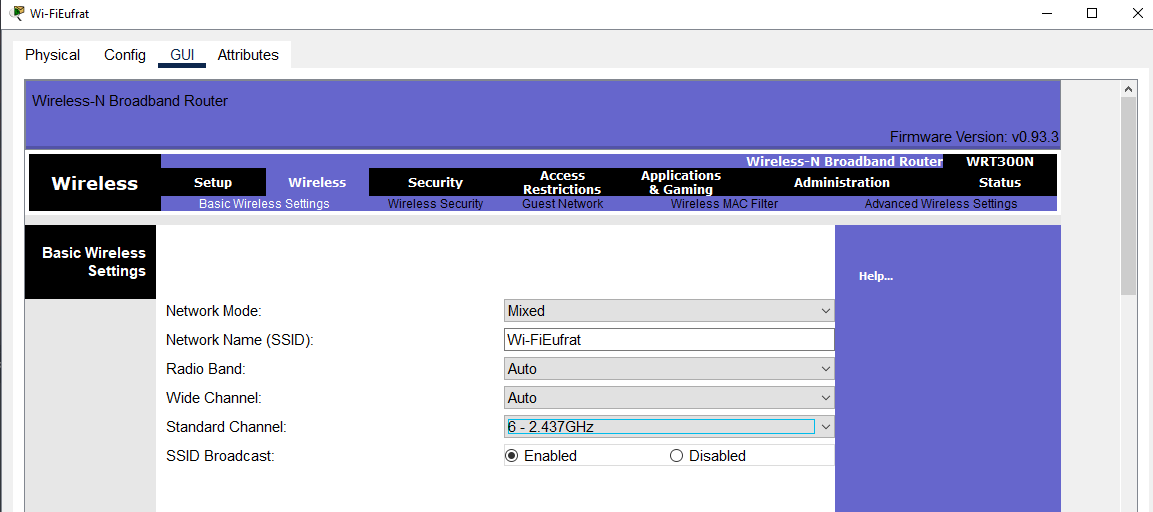
\includegraphics[width=0.75\linewidth]{Wireless.png}
\end{center}

\begin{itemize}
    \item Network Mode $\rightarrow$ Mixed
    \item Network Name (SSID)$\rightarrow$ Wi-FiOras
    \item Radio Band $\rightarrow$Auto
    \item Wide Channel $\rightarrow$ Auto
    \item Standard Channel $\rightarrow$ alegem fie 6 fie 11
    \item SSID Broadcast $\rightarrow$ Enable
    \item \underline{Scroll jos de tot $\rightarrow$ Save Settings}
\end{itemize}
\begin{center}
    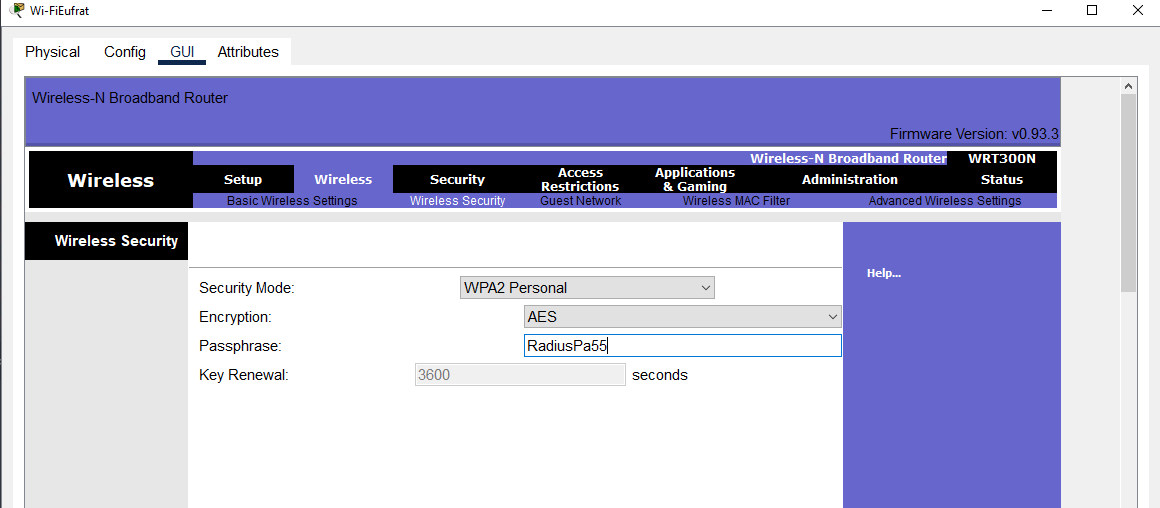
\includegraphics[width=0.75\linewidth]{Wireless Security.png}
\end{center}
Subtab Wireless Security


\begin{itemize}
    \item Security Mode $\rightarrow$WPA2Personal
    \item Encryption $\rightarrow$AES
    \item Passphrase $\rightarrow$ RadiusPa55
    \item \underline{Scroll jos de tot$\rightarrow$Save Settings}
\end{itemize}

\subsubsection{Wifi Laptops}


Acum mai trebuie sa aducem dispozitive pe care sa le conectam la reteaua Wi-Fi, adica laptopuri.

End Devices $\rightarrow$ End Devices $\rightarrow$ Laptop

Pentru prima data vom folosi aici tab-ul Physical:

$\rightarrow$ Power OFF Laptop button $\rightarrow$ Luam placa de retea $\rightarrow$ Modules $\rightarrow$ WPC300N $\rightarrow$ Introducem $\rightarrow$ Power On

Click Laptop $\rightarrow$ Desktop $\rightarrow$ PC Wireless 

\begin{center}
    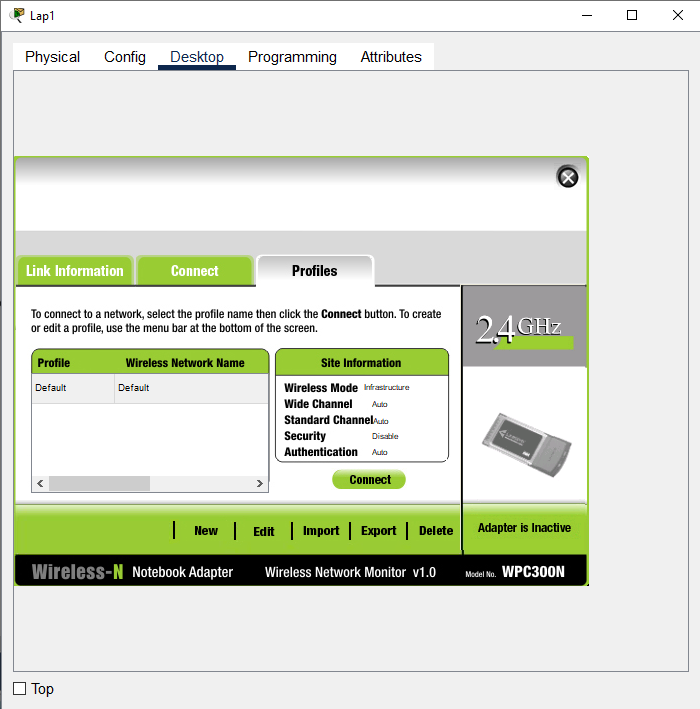
\includegraphics[width=1\linewidth]{Profiles.png}
\end{center}

Profiles $\rightarrow$ New $\rightarrow$ \textbf{Wi-FiOras} $\rightarrow$ Advanced Setup 

Infrastructure Mode $\rightarrow$Wireless Network Name (SSID) $\rightarrow$ \textbf{Wi-FiOras} $\rightarrow$ Next

Obtain Network Settings Automatically (DHCP) $\rightarrow$ Next $\rightarrow$

Security $\rightarrow$ WPA2-Personal $\rightarrow$

Pre-Shared Key $\rightarrow$ \textbf{RadiusPa55} $\rightarrow$ Next $\rightarrow$ Save $\rightarrow$ Connect to Network


Reteaua de Wi-Fi ar trebui sa apara la Profiles.

\begin{center}
    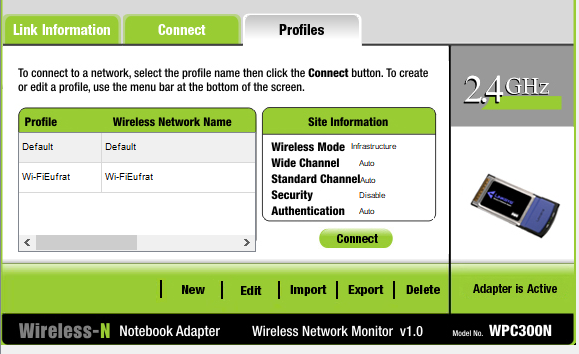
\includegraphics[width=0.75\linewidth]{Connected.png}
\end{center}

Dupa ce ne-am conectat putem sa verificam daca laptopurile primesc IP in mod dinamic prin DHCP

\begin{center}
    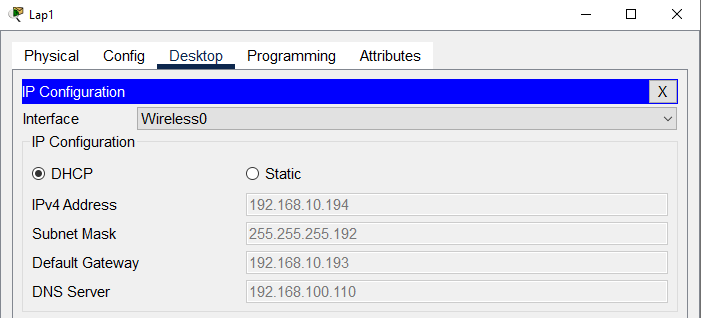
\includegraphics[width=0.75\linewidth]{DHCP.png}
\end{center}

\subsubsection{MAC Filtering}
Spre finalul laboratorului s-ar putea sa va fie predat putin pe graba inca un concept mai important dar nu foarte folosit, "Filtrarea pe adrese MAC".

Cand esti conectat de pe laptop la WiFi-Router $\rightarrow$
\newline 
Wireless $\rightarrow$ Wireless MAC Filter $\rightarrow$ Enabled  $\rightarrow$ Permit PCs...access

Ce urmeaza este sa setam un Whitelist/Blacklist de adrese MAC unde vom decide precis ce dispozitive vrem sa se conecteze la reteaua de WiFi sau care nu. Adresa MAC trebuie introdusa manual.

\begin{center}
    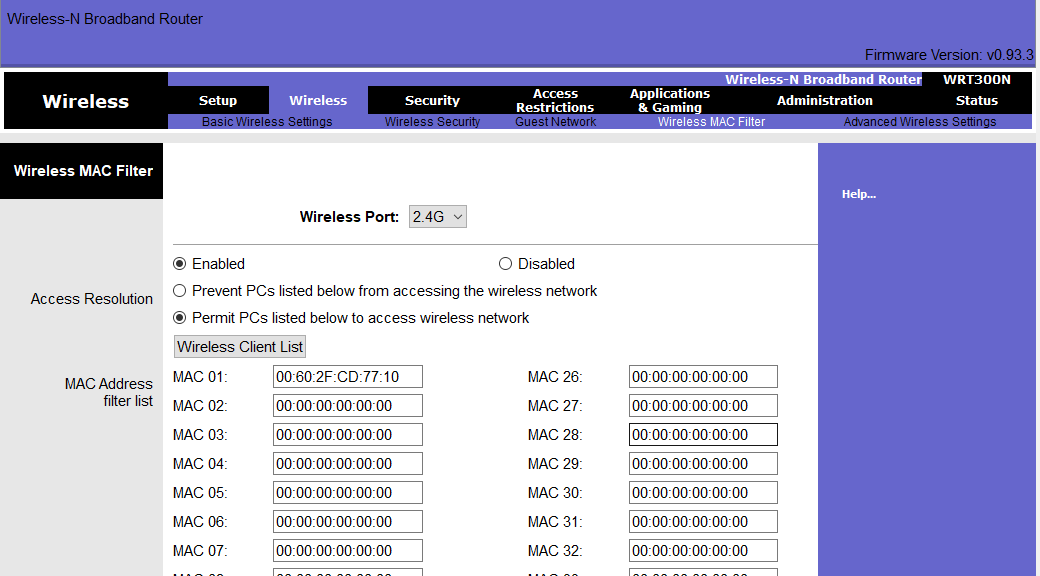
\includegraphics[width=1\linewidth]{MACFilter.png}
\end{center}

Urmeaza sa aducem un nou laptop pe spatiul de lucru, ii vom pune modulul de internet WPC300N, si ii vom afla adresa MAC ca pe un dispozitiv cu OS Windows.

Scopul este ca unul dintre laptopuri sa se poata conecta liber la retea, celalalt sa nu se poata conecta oricat de mult incearca!

De preferat este sa facem un whitelist in loc de blacklist.

1. Mereu vom avea un inventar al dispozitivelor autorizate pentru a se contecta la retea.

2. Dispozitivele virtuale care nu au deloc adresa MAC nu se pot conecta

3. Este un strat de securitate in plus
\begin{center}
    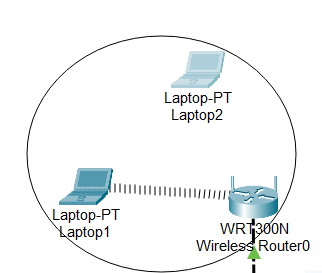
\includegraphics[width=0.5\linewidth]{MACFilteredWiFi.png}
\end{center}

\newpage

Lap2 $\rightarrow$ Desktop $\rightarrow$ Command Prompt $\rightarrow$ ipconfig /all $\rightarrow$ Physical Address 

\begin{center}
    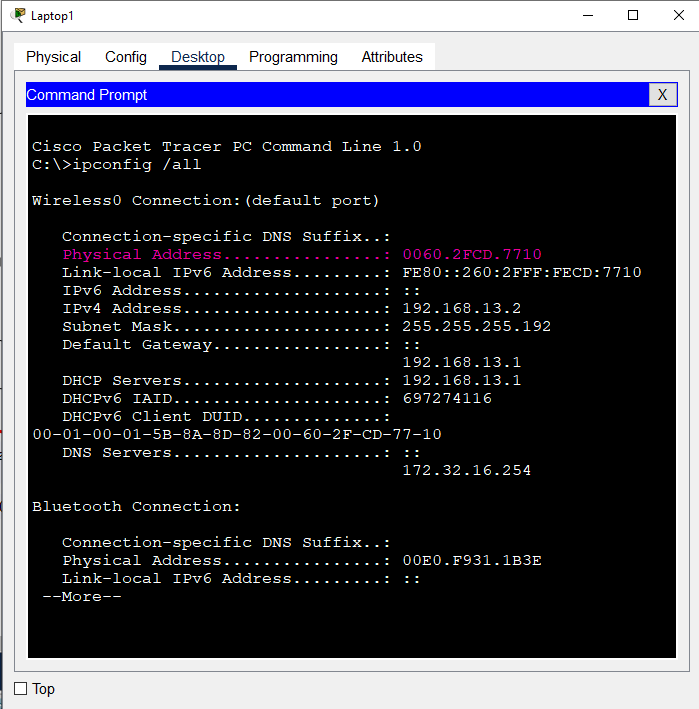
\includegraphics[width=1\linewidth]{ipconfigMAC.png}
\end{center}




\subsubsection{Conexiune Exterior}

Ca sa putem spune ca am terminat de configurat router-ul Wi-Fi, trebuie sa verificam ca este posibil să dăm ping de la oricare echipament din interiorul rețelei Wi-Fi, către oricare echipament din exteriorul rețelei Wi-Fi.

Iar deoarece rețeaua Wi-Fi este privata, echipamentele din exterior nu pot da ping explicit (deoarece ar putea fi o multitudine de router-e Wi-Fi toate cu ip-ul intern 192.168.0.1), dar pot să răspundă la ping-uri și să inițieze conversație cu echipamentele din rețeaua Wi-Fi prin serviciul de Email.


Pentru asta, trebuie să avem în vedere:

 Ca fiecare router să știe ruta spre subrețeaua care leagă R-WiFi de Router-ul cel mai apropiat, prin rutare statică din aproape in aproape.
    
(aici 10.10.10.0/30)

\begin{verbatim}
#R-Eufrat70(config)#ip route 10.10.10.0 255.255.255.252 A.B.C.D
\end{verbatim}



\section{Cabluri. Legaturi. Porturi.}
\subsection{Placile de Retea}
Reamintim ca pe PC si pe Server trebuie sa schimbam placa de retea dintr-una cu port de FastEthernet cu una de GigabitEthernet. (well nu TREBUIE, dar trebuie).

Pentru Router trebuie sa adaugam cele 2 porturi serial.

\paragraph{PC}:
Click PC $\rightarrow$ Physical $\rightarrow$Power Off$\rightarrow$ Drag \& Drop $\rightarrow$ luam placa de retea $\rightarrow$ Drop at Modules $\rightarrow$ luam PT-HOST-NM-1CGE $\rightarrow$ punem in slot $\rightarrow$ Power On

\paragraph{Server}:
Click Server $\rightarrow$ Physical $\rightarrow$ Click Power Off $\rightarrow$ Luam placa ce era deja sus$\rightarrow$Drag\&Drop$\rightarrow$Drop at Modules $\rightarrow$luam PT-HOST-NM-1CGE$\rightarrow$ punem in slot-ul de sus.$\rightarrow$Power On

\paragraph{Router}:
Click Router $\rightarrow$ Physical $\rightarrow$Power Off$\rightarrow$ Drag \& Drop $\rightarrow$ luam placa de retea $\rightarrow$ Drop at Modules $\rightarrow$ luam HWIC-2T $\rightarrow$ punem in al 4-lea slot, in dreapta sus langa sursa $\rightarrow$ Power On



\subsection{Ce. Cu cine. Unde.}
Tea.You.Anywhere.

Cablurile se gasesc in:
Stanga jos $\rightarrow$ Connections$\rightarrow$ Connections. 

\begin{itemize}
    \item \textbf{Laptop numit SERVICE - Switch/Router} $\rightarrow$ cablu Console 

    $\rightarrow$ SERVICE $\rightarrow$ port RS232

    $\rightarrow$ Switch/Router $\rightarrow$ port Console

    \item \textbf{PC - Switch}  $\rightarrow$ Copper Straight-Through. 

    $\rightarrow$ PC $\rightarrow$ port GigabitEthernet 0
    
    $\rightarrow$ Switch $\rightarrow$ port FastEthernet \{0-24\}

    *nu prea conteaza, dar o conventie ar putea fi ca pe cele 24 porturi FA sa punem PC-uri si pe cele 2 GIGA sa punem legaturile speciale.

    \item \textbf{Switch - Router} $\rightarrow$ Copper Straight-Through
    
    $\rightarrow$ Switch $\rightarrow$ port GigabitEthernet \{1/2\}
    
    $\rightarrow$ Router $\rightarrow$ port GigabitEthernet 0
    \item \textbf{Router - Router} $\rightarrow$ Serial DTE
    
    $\rightarrow$ Router1 $\rightarrow$ port Serial 0/0/0
    
    $\rightarrow$ Router2 $\rightarrow$ port Serial 0/0/0
     
    *incercam sa avem ambele routere pe acelasi Serial, fiindca e mai usor de tinut minte, daca apare un al 3-lea router, intram pe Serial 0/0/0

    \item \textbf{Server - Switch} Copper Straight-Through

    $\rightarrow$ Server $\rightarrow$ port GigabitEthernet 0

    $\rightarrow$ Switch $\rightarrow$ port GigabitEthernet \{1/2\} (i guess merge oricum oricare si FA dar idk)
    
    

    



   
    \item \textbf{Router - Server} Copper Straight-Through

    $\rightarrow$ Router $\rightarrow$ port GigabitEthernet 0/1/2

    $\rightarrow$ Server $\rightarrow$ port GigabitEthernet 0

     *nu e nevoie sa legam serverul direct la router, adia putem si prin switch, dar uneori la lab se cere direct la router.

    \item \textbf{Laptop numit SERVICE - Wi-Fi Router} Copper Straight-Through

    $\rightarrow$ SERVICE $\rightarrow$ port FastEthernet 0

    $\rightarrow$ Wi-Fi Router $\rightarrow$ port Internet 1

    \item \textbf{Wi-Fi Router - Router}$\rightarrow$ \underline{Copper Cross-Over}

    $\rightarrow$ Wi-Fi Router $\rightarrow$ port Internet (simplu, nu 1-5)

    $\rightarrow$ Router $\rightarrow$ port GigabitEthernet 1 (fiindca GIGA 0 va fi legat de switch)
\end{itemize}

\section{Explicatie comenzi}



\subsection{Helper}
Deoarece echipamentele cu care lucram noi (switch-uri. routere etc) nu au toate (sau nu au mereu) interfata grafica GUI, ce vom face mai mereu va fi sa luam un laptop, sa il numim SERVICE, (dar eu prefer LAPTOP DE LA DIGI), sa il conectam cu un cablu CONSOLE pe portul RS232 de laptop, respectiv portul consola pe echipament, si din laptop sa configuram echipamentul respectiv.

De mentionat ca tot un CLI (Command Line Interface) este, si daca ai trecut de laboratorul de sisteme de operare, iti va fi ok, iar terminalul va urla (dar nu e garantat) daca nu ai scris o comanda cum trebuie.

Daca ai vreodata dubii la cum era sintaxa vreunei comenzi, foloseste helperul scriind simbolul de "?" !!!!

eg.
\begin{verbatim}
Router#clo?
clock
Router#clock ?
  set Set the time and date
Router#clock set ?
  hh:mm:ss Current Time
\end{verbatim}

De asemeni jucati-va cu tasta Tab.

\subsection{Comenzi}

\begin{itemize}

\item 
\begin{verbatim}
Switch>enable
\end{verbatim}
Trecem din normal user mode in privileged user mode. 

\item
\begin{verbatim}
Switch#configure terminal
\end{verbatim}
Trecem din privileged mode in global-config mode.

\item
\begin{verbatim}
Switch#no ip domain lookup
\end{verbatim}
Prin default, de fiecare data cand introducem text in CLI, daca acel text nu este o comanda corecta de Cisco (adica atunci cand gresim noi o comanda), switch-ul va crede ca noi am incercat sa scriem un domain name (eg. old.fmi.unibuc.ro) si va sta sa caute acel domain prin amintrilile sale, si nu prea ne ajuta sa vedem:
\begin{verbatim}
    Translating "old.fmi.unibuc.ro"...domain server(255.255.255.255)
\end{verbatim}
Deci mai bine dezactivam acest lucru cand configuram switch-ul. 

\item 
\begin{verbatim}
Sw_CRIS(config)#no cdp run
\end{verbatim}
cdp = Cisco Discovery Protocol. 

Aparent, la fiecare 60 de secunde (configurabil) sau cand se transmit pachete normale, dispozitivele Cisco isi transmit si mesaje aditionale intre ele. Mesaje care contin informatii despre software, hardware, detalii de productie, in cate secunde sa stearga pachetul acesta de date, etc. Scopul este identificarea si comunicarea intre vecinii din retea pentru posibile re-rutari mai tarzii in retea daca, sa zicem, pica un router. 

Deci hai sa dezactivam asta pentru securitate.

\item
\begin{verbatim}
Sw_CRIS(config)#service password-encryption
\end{verbatim}
Activeaza serviciul de criptare a parolelor. Intuitiv ar fi sa facem asta inainte sa setam parolele.

In Cisco anumite drepturi si actiuni pot fi limitate prin conceptul de `privilege`. Privilegiile sunt pe nivele, si exita un total de 16 (numerotate 0-15, crescator precum gradul de access). De fiecare data cand setam o parola, putem sa mai punem un parametru {level X} ca sa setam privilegiile pe care le ofera parola aceea drept X. In mod default parolele au privilege 15.
\begin{itemize}
    \item{level 0:} are access doar la 5 comenzi: logout, enable, disable, help, exit. 
    \item{level 15:} privileged EXEC mode user
\end{itemize}

\item
\begin{verbatim}
Sw_CRIS(config)#enable password ciscoenapa55
Sw_CRIS(config)#enable secret ciscosecpa55
\end{verbatim}
Definim sau redefinim o parola, respectiv o parola \underline{secreta} encriptata non-reversibil diferit, care au rolul de a da acces la privileged EXEC mode.


\item
\begin{verbatim}
Sw_CRIS(config)#banner motd #mesaj#
\end{verbatim}
Punem un banner de tip `Message of the Day` care va fi afisat la login.
Are un maxim 80 de caractere si captureaza tot textul dintre 2 simboluri oarecare, cu conditia ca mesajul sa inceapa si sa se termine cu acel simbol (aici \# in cod \%, sau orice altceva)

\item
\begin{verbatim}
Sw_CRIS(config)#line console 0
Sw_CRIS(config-line)#password ciscoconpa55
Sw_CRIS(config-line)#login
Sw_CRIS(config-line)#logging synchronous
Sw_CRIS(config-line)#exec-timeout 20 10
Sw_CRIS(config-line)#exit
\end{verbatim}
Din global config intram in (config-line)\# adica pe consola, apoi configuram cadrul de logare prin parola locala si sincrona. Adica limitam accesul la alte reconfigurari prin cablu consola (ceea ce facem si noi acum).

\item
\begin{verbatim}
exec-timeout 20 10
\end{verbatim} va incheia conexiunea automat dupa 20 de minute si 10 secunde (secundele sunt optionale).

\item 
\begin{verbatim}
Sw_CRIS#copy running-config startup-config
sau
Sw_CRIS#copy run start
\end{verbatim}
Salvam configuratiile de sistem de pana acum adaugandu-le la configuratiile de startup. Pe switch ar trebui sa existe un fisier local de startup-config, si noi doar adaugăm acolo modificarile pe care le-am facut pana acum, astfel atunci cand switch-ul isi da reboot, nu va uita de modificarile noastre. Este util ca sa nu ne pierdem munca. Asta se aplica si dacă doar se ia curentul, deoarece Running-Config se afla in RAM si Startup-Config în NVRAM. (non-volatile)

*Totodată merge pe toate echipamentele.

\item 
\begin{verbatim}
Sw_CRIS#clock set 14:45:15 5 Mar 2025
\end{verbatim}
Setam ceasul local de pe switch. 
Formatul este 

clock set hh:mm:ss day month year

De mentionat ca luna se scrie cu text in engleza, nu neaparat prescurtat sau majuscule.

\item 
\begin{verbatim}
Sw_CRIS(config)#username Admin01 privilege 15 secret Admin01pa55
\end{verbatim} 
Creem un cont de utilizator numit Admin01, ii dam privilegii maxime, si parola sa o setam Admin01pa55, pe aceasta o folosim cand ne logam prin ssh.

\item 
\begin{verbatim}
Switch(config)#hostname Sw_CRIS
...
Sw_CRIS(config)#ip domain name info.ro
Sw_CRIS(config)#crypto key generate rsa
>2048>enter
\end{verbatim} 
Generam o cheie de securitate pe algoritmul RSA. (Suntem obligati sa avem setate si un Hostname si un IP domain name inainte de asta!) Lungimea o setam pe 2048 bytes.

RSA vine de la Rivest–Shamir–Adleman.

\url{https://en.wikipedia.org/wiki/RSA_cryptosystem}.




\item 
\begin{verbatim}
Sw_CRIS(config)#ip ssh version 2
...
Sw_CRIS(config)#line vty 0 15
Sw_CRIS(config-line)#transport input ssh
\end{verbatim}

VTY = Virtual Teletype

Pe linia consola vty, activam protocolul de conexiune prin ssh.


\item 
\begin{verbatim}
Sw_CRIS(config)#logging host 209.165.200.190
Sw_CRIS(config)#service timestamps log datetime msec
Sw_CRIS(config)#service timestamps debug datetime msec
\end{verbatim}
Toate actiunile facute pe acest dispozitiv for fi scrise si trimise serverului de pe adresa 209.165.200.190 pentru debug/contabilitate/tracing/digital footprint/accountability etc


\item 
\begin{verbatim}
Sw_CRIS(config)#interface vlan 1
Sw_CRIS(config-if)#ip address 172.32.40.2 255.255.248.0
Sw_CRIS(config-if)#no shutdown
Sw_CRIS(config-if)#exit
\end{verbatim}

Arguably cea mai importanta (sau singura importantă) parte, sa asociem switch-ului nostru o adresa IP cu tot cu masca.

Prin `no shutdown` ne asiguram ca linia de comunicare virtuala ramane activa si portul accepta mesaje până pică.


\item 
\begin{verbatim}
R-Anglia(config)#ip route 209.100.100.160 255.255.255.224 10.10.10.10
sau 
R-Anglia(config)#ip route 209.100.100.160 255.255.255.224 serial 0/0/X
\end{verbatim}
unde $X\in\{0,1\}$

Permite routerului sa comunice cu Reteaua 209.100.100.160/27 prin adresa serial 10.10.10.10/30 cu care este legat (pe Serial 0/0/0, lab3)

\item 
\begin{verbatim}
C:\>ftp 209.100.100.190
\end{verbatim}

(Lab4.) Ne conectam din Anglia sau Franta la server prin serviciul de FTP. ftp + adresa serverului.



\end{itemize}
\newpage


\section{Cod laboratoare}
Aici se vor afla pe de-o parte, paginile de cod care au fost predate la laborator, pe de alta parte, indicatii + adrese, si pe de alta parte, retusuri facute de mine pentru claritate / sens.

\subsection{Lab2 Config Switch}
\subsubsection{Cod}

Click PC$\rightarrow$Desktop$\rightarrow$Ip Configuration

\begin{center}
    IP Configuration PC CRIS
\end{center}
\begin{center}
    \begin{tabular}{|c|c|}\hline
         Static & (Bifat)  \\ \hline \hline
         IP & 172.32.40.81  \\ \hline
         Subnet Mask & 255.255.248.0 \\ \hline
         Default Gateway & 172.32.40.1 \\ \hline
         DNS Server & 209.165.200.190 \\ \hline
    \end{tabular}
\end{center}

Click PC$\rightarrow$Desktop$\rightarrow$Email

\begin{center}
    Email PC
\end{center}
\begin{center}
    \begin{tabular}{|c|c|}\hline
         Your Name & CRIS  \\ \hline 
         Email Address & CRIS@info.ro  \\ \hline
         Incoming Mail Server & 209.165.200.190 \\ \hline
         Outgoing Mail Server & 209.165.200.190 \\ \hline
         Username & CRIS \\ \hline
         Password & 123456 \\ \hline

    \end{tabular}
\end{center}
\newpage
\begin{verbatim}
    Switch>enable
    Switch#configure terminal
    Switch(config)#no ip domain lookup
    Switch(config)#hostname Sw_CRIS
    Sw_CRIS(config)#no cdp run
    Sw_CRIS(config)#service password-encryption
    Sw_CRIS(config)#enable secret ciscosecpa55
    Sw_CRIS(config)#enable password ciscoenapa55
    Sw_CRIS(config)#banner motd %Luni 10.03.2025 Sedinta IT, free coffee!%
    Sw_CRIS(config)#line console 0
    Sw_CRIS(config-line)#password ciscoconpa55
    Sw_CRIS(config-line)#login
    Sw_CRIS(config-line)#logging synchronous
    Sw_CRIS(config-line)#exec-timeout 20 10
    Sw_CRIS(config-line)#exit
    Sw_CRIS(config)#line vty 0 15
    Sw_CRIS(config-line)#password ciscovtypa55
    Sw_CRIS(config-line)#login
    Sw_CRIS(config-line)#logging synchronous
    Sw_CRIS(config-line)#exec-timeout 5 10
    Sw_CRIS(config-line)#exit
    Sw_CRIS(config)#exit 
    Sw_CRIS#copy running-config startup-config
    >enter
    Sw_CRIS#clock set 14:45:15 5 Mar 2025
    Sw_CRIS#configure terminal
    Sw_CRIS(config)#ip domain name info.ro
    Sw_CRIS(config)#username Admin01 privilege 15 secret Admin01pa55
    Sw_CRIS(config)#line vty 0 15
    Sw_CRIS(config-line)#transport input ssh
    Sw_CRIS(config-line)#login local
    Sw_CRIS(config-line)#exit
    Sw_CRIS(config)#crypto key generate rsa
    >2048>enter
    Sw_CRIS(config)#ip ssh version 2
    Sw_CRIS(config)#logging host 209.165.200.190
    Sw_CRIS(config)#service timestamps log datetime msec
    Sw_CRIS(config)#service timestamps debug datetime msec
    Sw_CRIS(config)#interface vlan 1
    Sw_CRIS(config-if)#description #Legatura ramura 172.32.40.0#
    Sw_CRIS(config-if)#ip address 172.32.40.2 255.255.248.0
    Sw_CRIS(config-if)#no shutdown
    Sw_CRIS(config-if)#exit
    Sw_CRIS(config)#ip default-gateway 172.32.40.1
\end{verbatim}

\newpage
\subsubsection{Testare}
Iar pentru a testa configuratia curenta.

CRIS $\rightarrow$ Desktop $\rightarrow$  Command Prompt (CMD)

\begin{verbatim}
    Cisco Packet Tracer PC Command Line 1.0
    C:\>ping 172.32.40.2
    Request timed out.
    Reply from 172.32.40.2: bytes=32 time<1ms TTL=255
    Reply from 172.32.40.2: bytes=32 time<1ms TTL=255
    Reply from 172.32.40.2: bytes=32 time<1ms TTL=255

    C:\>ssh -l Admin01 172.32.40.2
    >Admin01pa55
\end{verbatim}


Pentru ping, se vor trimite 4 pachete de date, daca am facut totul ok, atunci ne asteptam ca primul pachet va fi pierdut pe drum, dar celelalte 3 vor fi primite, si conexiunea va deveni stabila pentru ping-uri ulterioare.

Daca s-au pierdut toate pachetele, atunci trebuiesc verificate configurarile de ip pentru PC si pentru Switch. 

Pentru logarea prin ssh, vom incerca sa ne conectam prin contul facut mai devreme de admin, cu privilegii maxime de user EXEC mode.

Daca nu am avea privilege 15 atunci, la incercarea de a accesa unele interfete sau linii, cum am facut pana acum, ni s-ar cere parolele pe care le-am setat pe consola, vty, si pe global settings mode.

Pagina urmatoare contine acelasi cod dar reformatat deoarece consider ar avea mai mult sens daca unele comenzi ar fi in alta ordine, si nu am iesi din mijlocul configurarii liniei vty 0 15 doar ca sa setam ceasul si sa facem un cont.
\newpage
\subsubsection{Cod dar rescris}

\begin{verbatim}
    Switch>enable
    SwitchS#clock set 14:45:15 5 Mar 2025
    Switch#configure terminal
    Switch(config)#no ip domain lookup
    Switch(config)#no cdp run
    Switch(config)#hostname Sw_CRIS
    Sw_CRIS(config)#service password-encryption
    Sw_CRIS(config)#enable secret ciscosecpa55
    Sw_CRIS(config)#enable password ciscoenapa55
    Sw_CRIS(config)#ip domain name info.ro
    Sw_CRIS(config)#ip default-gateway 172.32.40.1
    Sw_CRIS(config)#crypto key generate rsa
    >2048>enter
    Sw_CRIS(config)#ip ssh version 2
    Sw_CRIS(config)#logging host 209.165.200.190
    Sw_CRIS(config)#service timestamps log datetime msec
    Sw_CRIS(config)#service timestamps debug datetime msec
    Sw_CRIS(config)#username Admin01 privilege 15 secret Admin01pa55
    Sw_CRIS(config)#banner motd %Luni 10.03.2025 Sedinta IT, free coffee!%
    Sw_CRIS(config)#line console 0
    Sw_CRIS(config-line)#password ciscoconpa55
    Sw_CRIS(config-line)#login
    Sw_CRIS(config-line)#logging synchronous
    Sw_CRIS(config-line)#exec-timeout 20 10
    Sw_CRIS(config-line)#exit
    Sw_CRIS(config)#line vty 0 15
    Sw_CRIS(config-line)#password ciscovtypa55
    Sw_CRIS(config-line)#login local
    Sw_CRIS(config-line)#logging synchronous
    Sw_CRIS(config-line)#exec-timeout 5 10
    Sw_CRIS(config-line)#transport input ssh
    Sw_CRIS(config-line)#exit
    Sw_CRIS(config)#interface vlan 1
    Sw_CRIS(config-if)#description #Legatura ramura 172.32.40.0#
    Sw_CRIS(config-if)#ip address 172.32.40.2 255.255.248.0
    Sw_CRIS(config-if)#no shutdown
    Sw_CRIS(config-if)#exit

    (de mentionat ca de salvat, salvezi cand vrei, 
    dar hai nu in mijlocul configurarii SSH ca ai uitat sa setezi ceasul)
    Sw_CRIS(config)#exit 
    Sw_CRIS#copy running-config startup-config
    >enter
    Sw_CRIS#configure terminal
\end{verbatim}

\subsection{Lab3 Config Router + Server}
*Note..dupa cateva calcule....adresele din ramura de Server din notite imi par gresite, sunt 99.9\% sigur ca R-Server ar trebui sa aiba NA 209.100.100.160, deoarece DGW 209.100.100.129 nu are sens, range prea mic pentru a include serverul. Deci ce urmeaza este si putin improvizat dar corect.

Presupunem 2 PC-uri numite frumos, Anglia si Franta, care pot sa comunice prin Email.

Dar aceste pc-uri apartin de retele diferite:

\begin{itemize}
    \item Retea Anglia. NA = 192.168.50.32/27
    \item Retea Franta. NA = 209.100.100.160/27
\end{itemize}


\begin{figure}
    \centering
    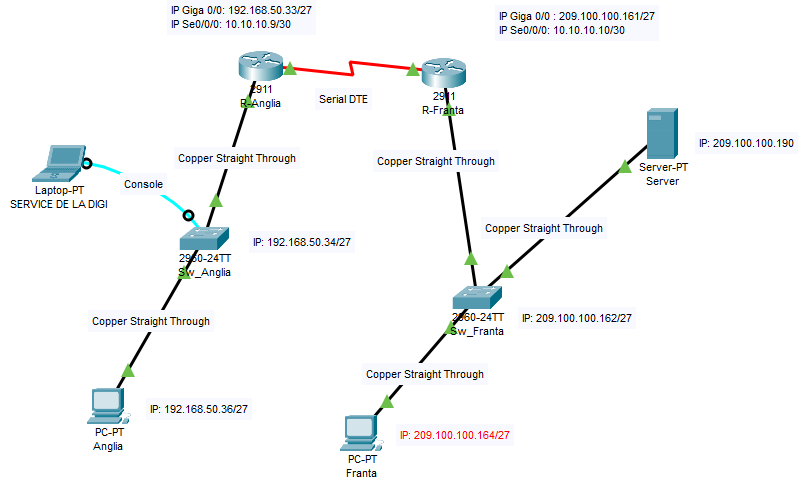
\includegraphics[width=1\linewidth]{Screenshot 2025-04-04 112721.png}
    \caption{Lab3}
\end{figure}

\newpage
\subsubsection{Config router}
\paragraph{Locatie Router}:

(Stanga Jos)$\rightarrow$ Network Devices $\rightarrow$ Routers $\rightarrow$ 2901 si \underline{2911} $\rightarrow$Drag\&Drop$\rightarrow$Spatiu de lucru$\rightarrow$Schimbam numele.

Si 2901 si 2911 sunt optiuni bune dar recomandarea este sa folosim 2911.

\paragraph{Startup Router}:

Left Click Router $\rightarrow$ Physical $\rightarrow$ Click Power Off button $\rightarrow$ Luam placa HWIC-2T $\rightarrow$Drag\&Drop$\rightarrow$punem in slot-ul cat mai aproape de sursa (dreapta sus).$\rightarrow$Click power on.


\subsubsection{Config Server}


\paragraph{Locatie Server}:

(Stanga Jos) $\rightarrow$ End Devices $\rightarrow$ End Devices $\rightarrow$ Server$\rightarrow$ Drag\&Drop$\rightarrow$Spatiu de lucru$\rightarrow$Schimbam numele.

\paragraph{Startup Server}:

Left Click Server $\rightarrow$ Physical $\rightarrow$ Click Power Off button $\rightarrow$ Luam placa ce era deja sus$\rightarrow$Drag\&Drop$\rightarrow$Drop at Modules $\rightarrow$Take PT-HOST-NM-1CGE$\rightarrow$ punem in slot-ul de sus.$\rightarrow$Turn on button

\subsubsection{Services}

Tab Services $\rightarrow$ Vezi module stanga.

\begin{itemize}
    \item HTTP
        \begin{itemize}
            \item  HTTP $\rightarrow$ (BIFAT OFF)
            \item  HTTPS $\rightarrow$ (BIFAT ON)
        \end{itemize}
    \item DNS
        \begin{itemize}
            \item DNS Service $\rightarrow$ (BIFAT ON)
            \item Name $\rightarrow$ info.ro
            \item Address $\rightarrow$ 209.100.100.190
            \item Type $\rightarrow$ A record
            \item Add
        \end{itemize}
    \item Email
        \begin{itemize}
            \item Domain Name $\rightarrow$ info.ro
            \item Set
            \item User $\rightarrow$ `Nume user`
            \item Password $\rightarrow$ 123456
            \item Press + button. Adaugam fiecare utilizator (adica user PC), server inclusiv.
        \end{itemize}
        \newpage
    \item Syslog
        \begin{itemize}
            \item Service $\rightarrow$ (BIFAT ON)
            \item aici o sa ne vedem inregistrarile samd.
            \item tine minte 3 cuvinte: Authentification Acreditation Accounting
        \end{itemize}
    \item FTP
        \begin{itemize}
            \item Service $\rightarrow$ (BIFAT ON)
            \item Username $\rightarrow$ Anglia
            \item Password $\rightarrow$ 123456
            \item Write Read Delete Rename List Rights
            \item Add (Facem cont pentru toti userii, adica fiecare PC)
        \end{itemize}

    

    
\end{itemize}



\subsubsection{Inputs}
Click PC$\rightarrow$Desktop$\rightarrow$Ip Configuration

\begin{center}
    IP Configuration PC Anglia
\end{center}
\begin{center}
    \begin{tabular}{|c|c|}\hline
         Static & (Bifat)  \\ \hline \hline
         IP & 192.168.50.36  \\ \hline
         Subnet Mask & 255.255.255.224 \\ \hline
         Default Gateway & 192.168.50.33 \\ \hline
         DNS Server & 209.100.100.190 \\ \hline
    \end{tabular}
\end{center}


\begin{center}
    IP Configuration PC Franta
\end{center}
\begin{center}
    \begin{tabular}{|c|c|}\hline
         Static & (Bifat)  \\ \hline \hline
         IP & 209.100.100.164  \\ \hline
         Subnet Mask & 255.255.255.224 \\ \hline
         Default Gateway & 209.100.100.161 \\ \hline
         DNS Server & 209.100.100.190 \\ \hline
    \end{tabular}
\end{center}

Click PC$\rightarrow$Desktop$\rightarrow$Email

\begin{center}
    Email PC Anglia
\end{center}
\begin{center}
    \begin{tabular}{|c|c|}\hline
         Your Name & Anglia  \\ \hline 
         Email Address & Anglia@info.ro  \\ \hline
         Incoming Mail Server & 209.100.100.190 \\ \hline
         Outgoing Mail Server & 209.100.100.190 \\ \hline
         Username & Anglia \\ \hline
         Password & 123456 \\ \hline
    \end{tabular}
\end{center}


\begin{center}
    Email PC Franta
\end{center}
\begin{center}
    \begin{tabular}{|c|c|}\hline
         Your Name & Franta  \\ \hline 
         Email Address & Franta@info.ro  \\ \hline
         Incoming Mail Server & 209.100.100.190 \\ \hline
         Outgoing Mail Server & 209.100.100.190 \\ \hline
         Username & Franta \\ \hline
         Password & 123456 \\ \hline
    \end{tabular}
\end{center}


Click Server$\rightarrow$Desktop$\rightarrow$Ip Configuration
\begin{center}
    IP Configuration Server
\end{center}
\begin{center}
    \begin{tabular}{|c|c|}\hline
         Static & (Bifat)  \\ \hline \hline
         IP & 209.100.100.190  \\ \hline
         Subnet Mask & 255.255.255.224 \\ \hline
         Default Gateway & 209.100.100.161 \\ \hline
         DNS Server & 209.100.100.190 \\ \hline
    \end{tabular}
\end{center}

Click Server$\rightarrow$Desktop$\rightarrow$Email

\begin{center}
    Email Configuration Server
\end{center}
\begin{center}
    \begin{tabular}{|c|c|}\hline
         Your Name & Server  \\ \hline 
         Email Address & Server@info.ro  \\ \hline
         Incoming Mail Server & 209.100.100.190 \\ \hline
         Outgoing Mail Server & 209.100.100.190 \\ \hline
         Username & Server \\ \hline
         Password & 123456 \\ \hline
    \end{tabular}
\end{center}

\subsubsection{Cod}
\begin{verbatim}



Sw_Anglia(config)#interface vlan 1
Sw_Anglia(config-if)#ip address 192.168.50.34
Sw_Anglia(config-if)#no shutdown
Sw_Anglia(config-if)#exit



Sw_Franta(config)#interface vlan 1
Sw_Franta(config-if)#ip address 209.100.100.162
Sw_Franta(config-if)#no shutdown
Sw_Franta(config-if)#exit



Router>enable
Router#configure terminal
Router(config)#no ip lookup domain
Router(config)#hostname R-Anglia
R-Anglia(config)#no cdp run
R-Anglia(config)#service password-encryption
R-Anglia(config)#security passwords min-length 10 (doar pe Router)
R-Anglia(config)#login block-for 75 attempts 3 within 10 (doar pe Router)
R-Anglia(config)#enable secret ciscosecpa55
R-Anglia(config)#enable password ciscoenapa55
R-Anglia(config)#banner motd ^Vineri 21.03.2025 la ora 12 serverul va fi oprit^
R-Anglia(config)#banner login &Accesul persoanelor neautorizate este strict interzis& (doar pe Router)
R-Anglia(config)#line console 0
R-Anglia(config-line)#password ciscoconpa55
R-Anglia(config-line)#login
R-Anglia(config-line)#logging synchronous
R-Anglia(config-line)#exec-timeout 20 15
R-Anglia(config-line)#exit
R-Anglia(config)#line vty 0 15
R-Anglia(config-line)#password ciscovtypa55
R-Anglia(config-line)#login
R-Anglia(config-line)#logging synchronous
R-Anglia(config-line)#exec-timeout 5 6
R-Anglia(config-line)#(CTRL+Z)
R-Anglia#copy running-config startup-config
>enter
R-Anglia#clock set 14:55:15 12 Mar 2025
R-Anglia#configure terminal
R-Anglia(config)#ip domain name info.ro
R-Anglia(config)#username Admin01 privilege 15 secret Admin01pa55
R-Anglia(config)#line vty 0 15
R-Anglia(config-line)#transport input ssh
R-Anglia(config-line)#login local
R-Anglia(config-line)#exit
R-Anglia(config)#crypto key generate rsa
>2048>enter
R-Anglia(config)#ip ssh version 2
R-Anglia(config)#logging host 209.100.100.190
R-Anglia(config)#service timestamps log datetime msec
R-Anglia(config)#service timestamps debug datetime msec
R-Anglia(config)#interface gigabitethernet 0/0
R-Anglia(config-if)#description Legatura cu reteaua 192.168.50.32/27 (Anglia)
R-Anglia(confif-if)#ip address 192.168.50.33 255.255.255.224
R-Anglia(config-if)#no shutdown
R-Anglia(config-if)#exit
R-Anglia(config)#ip route 209.100.100.160 255.255.255.224 10.10.10.10
R-Anglia(config)#interface serial 0/0/0
R-Anglia(config-if)#description Legatura cu routerul R-Server
R-Anglia(config-if)#ip address 10.10.10.9 255.255.255.252
R-Anglia(config-if)#no shutdown

de mentionat ca si R-Franta va fi configurat in mod practic identic, singura 
diferenta vor fi adresele, adica 3 comenzi vor fi diferite

R-Franta(config)#ip route 192.168.50.32 255.255.255.224 10.10.10.9
R-Franta(config)#interface gigabitethernet 0/0
R-Franta(config-if)#description Legatura cu reteaua 209.100.100.160/27 (Franta)
R-Franta(config-if)#ip address 209.100.100.161 255.255.255.224
R-Franta(config-if)#no shutdown
...
R-Franta(config)#interface serial 0/0/0
R-Franta(config-if)#description Legatura cu routerul R-Anglia
R-Franta(config-if)#ip address 10.10.10.10 255.255.255.252
R-Franta(config-if)#no shutdown

\end{verbatim}








\subsubsection{Testare}
\begin{itemize}

    \item[1.] Incearca sa dai ping de la PC-uri in celelalte componente. Din oricare pc in oricare componenta!

    \item[2.] Incearca sa dai un email din Anglia in Franta sa sugerezi ca vinul se bea mai bine cand te uiti la Courage the Cowardly dog.
        \begin{itemize}
            \item  To $\rightarrow$ Franta@info.ro
            \item  Subject $\rightarrow$ Recomandari
            \item  Mai tii minte cainele acela ce ne traumatiza pe cartoon network?
            \item Send
            \item Click Franta PC
            \item Email
            \item Receive \& Cry
        \end{itemize}
\newpage
\subsubsection{Serviciul FTP}
FTP = File Transfer Protocol.

TFTP = Trivial File Transfer Protocol (nu râde.)
\begin{itemize}
    \item[1.] Anglia $\rightarrow$ Desktop $\rightarrow$ Text Editor $\rightarrow$ Scriem un fisier si il salvam, sa zicem BugsBunny.txt.
    \item[2.] Verifica pe Anglia $\rightarrow$ Desktop $\rightarrow$ "TFTP Service" daca gasesti fisierul salvat.
    \item[3.] Desktop$\rightarrow$Command Prompt
    \item[4.] Daca ping-ul la server ne-a mers si am configurat corect serviciul de FTP:
    \item[5.]Hai sa ne conectam la server. Anglia $\rightarrow$ Command Prompt

    \begin{verbatim}
C:\>ftp 209.100.100.190
Trying to connect...
Connected to 209.100.100.190
220- Welcome to PT Ftp server
Username: Anglia
331- Username ok, need password
Password: 123456
230- Logged in
(passive mode On)
    \end{verbatim}
    \item[6.]Hai sa vedem toate comenzile.
    \begin{verbatim}
ftp>?
        ?            -this help
        cd           -change directory (duh)
        delete       -sterge fisier
        get          -descarca fisier (download)
        help         -this help
        passive      -toggle passive mode (habar n-am sincer ce este)
        put          -incarca fisier (upload)
        pwd          -print working directory
        quit         -incheie conexiunea
        rename       -deschide Super Smash Bros
    \end{verbatim}  
    \item[7.]Hai sa dam upload.

    \begin{verbatim}
        ftp>put BugsBunny.txt 
        
        Writing file BugsBunny.txt to 209.100.100.190:
    \end{verbatim}
    \item[8.]Hai sa descarcam ceva de pe server, poate contine parole de studenti sau anime-uri.
    \begin{verbatim}
        get ir800_yocto-1.7.2.tar 

        Reading file yr800_yocto-1.7.2.tar from 209.100.100.190:
        File transfer in progress...
    \end{verbatim}
    \item[9.] Anglia $\rightarrow$ Desktop$\rightarrow$TFTP Service$\rightarrow$ uite ce am gasit! 
\end{itemize}

    
    
\end{itemize}
DHCP = Dynamic Host Configuration Protocol

*gigabitethernet poate fi scris si prescurtat doar `giga` sau `gigabit`, dar terminalul nu este chiar 100$\%$ consistent pe asta

**in urma altor calcule, eu cred ca masca de pe subreteaua Server este gresita, o adresa 192.168.100.96/27, ar avea DNS = 192.168.100.126/27 si ca sa obtinem 192.168.100.110, masca ar trebui sa fie de /28, deci voi scrie ca atare, adica 255.255.255.240 nu 255.255.255.224 la R-Server

Concepte cabluri cu care se leaga router-router:
\begin{itemize}
    \item serial DTE: Data Terminal Equipment (folosim noi)
    \item serial DCE: Data Communication Equipment
\end{itemize}

\subsubsection{Cod}

\begin{verbatim}

(Configurare R-Eufrat)
---Leg de Eufrat---
R-Eufrat(config)#interface gigabitethernet 0/0
R-Eufrat(config-if)#description Legatura cu ramura Eufrat
R-Eufrat(config-if)#ip address 172.168.96.1 255.255.240.0
R-Eufrat(config-if)#ip helper-address 10.10.10.6
R-Eufrat(config-if)#no shutdown
R-Eufrat(config-if)#exit

---Leg de LAN Wi-Fi---
R-Eufrat(config)#interface gigabitethernet 0/1
R-Eufrat(config-if)#description Legatura cu R-Wi-Fi
R-Eufrat(config-if)#ip address 10.10.10.1 255.255.255.252
R-Eufrat(config-if)#no shutdown
R-Eufrat(config-if)#exit

---Leg de LAN Server---
R-Eufrat(config)#interface serial 0/0/0
(salvam, copy running-config startup-config)
R-Eufrat(config-if)#description Legatura cu R-Server
R-Eufrat(config-if)#ip address 10.10.10.5 255.255.255.252
R-Eufrat(config-if)#no shutdown 
R-Eufrat(config-if)#exit
R-Eufrat(config)#ip route 192.168.100.96 255.255.255.240 serial 0/0/0

(Configurare R-SERVER)
---Leg de LAN---
R-Server(config)#interface gigabitethernet 0/0
R-Server(config-if)#description Legatura cu Server
R-Server(config-if)#ip address 192.168.100.97 255.255.255.240
R-Server(config-if)#no shutdown
R-Server(config-if)#exit

---Leg de LAN Eufrat---
R-Server(config)#ip route 172.168.96.0 255.255.240.0 Serial 0/0/0
R-Server(config)#interface serial 0/0/0
R-Server(config-if)#description Legatura cu R-Eufrat
R-Server(config-if)#ip address 10.10.10.6 255.255.255.252
R-Server(config-if)#no shutdown
R-Server(config-if)#exit


(Putem testa din in host PC,ping + ssh, dupa ce am 
configurat vty 0 15 of course)
C:/>ping 172.168.96.2 (switch eufrat)
C:/>ping 172.168.96.1 (router eufrat)

\end{verbatim}

\subsubsection{Serviciul DHCP}
Dynamic Host Configuration Protocol.

Ca sa nu mai asignam noi ip-uri manual de fiecare data cand apare sau dispare sau arde vreun dispozitiv, putem sa alocam un pool de ip-uri, iar serverul local va aloca dinamic ip-uri.(adica va raspunde in timp real la ce se intampla in retea). Adica vedem ce se intampla daca la IP Configuration bifăm DHCP in loc de Static.

(DHCP, Eufrat)


Acum ca am stabilit o conexiune 3-way pe R-Eufrat(una cu subreteaua Eufrat si tot ce contine ea, una cu R-Server si ce contine el, si inca una cu R-WiFi), mai ramane doar sa configuram serviciul de DHCP in asa fel incat Serverul sa transmita adrese de IP prin routere catre R-Eufrat si el sa le aloce automat.


\paragraph{Ce adrese alocam?}

Adresele care sunt alocabile si nu sunt switch-uri. Adica trebuie sa calculam range-ul de switch-uri si sa vedem care este primul IP de host. Si apoi mai adaugam +1 special deoarece vom configura noi inca un PC mai "special" care va avea rol practic de "pilon" pentru adrese+testare.

Dupa cum sigur s-a observat, ramura Eufrat are masca 255.255.240.0, ceea ce inseamna o masca de 8+8+4=20 bits.
\[32-20 = 12\]

\[2^{12}-2=4094\]

\[\frac{4094}{26} \approx 157,46 \Rightarrow 158 \]

NA + 1 + 1 =  172.168.96.0/20 + 2 =  172.168.96.2/20 = primul switch

NA + 1 + 158 + 1 = 172.168.96.0/20 + 160 = 172.168.96.160/20 = adresa acelui PC special, imediat dupa ultimul switch

172.168.96.161/20 = prima adresa de PC-Host (care nu e setata special de noi)




\begin{verbatim}
---Prepar DHCP--- continuand comenzile de mai sus
R-Server(config)#ip dhcp excluded-address 172.168.96.1 172.168.96.160
R-Server(config)#ip dhcp pool Eufrat
R-Server(dhcp-config)#network 172.168.96.0 255.255.240.0
R-Server(dhcp-config)#default-router 172.168.96.1
R-Server(dhcp-config)#dns-server 192.168.100.110
R-Server(dhcp-config)#(CTRL+Z)
(save)
\end{verbatim}

Tot ce mai ramane este sa legam toate echipamentele, in special vom lega R-Eufrat de R-Server cu un cablu Serial DTE, la ambele capete pe portul Serial 0/0/0

Apoi adaugam primul PC din ramura Eufrat. Dar la IP Configuration vom bifa DHCP ON, si vedem ce se intampla.

\newpage
\subsubsection{RWi-Fi}
    acoperit in prezentare Echipament

\newpage
\section{Lab 6 Test}
\subsection{In prealabil}




\textbf{Foarte important} de notat este faptul ca la testul de laborator, NU avem voie cu nici un fel de materiale....sau hartie sau alte aplicatii software decat Cisco Packet Tracer...si asta include chiar până și aplicatia Calculator.

Ceea ce inseamna ca vom fi nevoiti sa facem calculele pe biti ADITIONALE pe notitele din CPT, ca sa si aflam reprezentarea in binar pentru octeti, acestea nu sunt punctate sau depunctate sau ceva, dar este cam singura cale.

Totodata pentru testul de laborator ni se cere sa avem pe ecran notite care sa urmareasca cei 3 pasi mari si lati din calcule. Acestea sunt singurele note-uri care trebuie neaparat sa fie pe ecran, restul sunt la latitudinea voastra... sau a cerintelor explicite.

In poza de mai jos, sub explicarea pasilor, sunt afisate toate calculele + toti pasii + alte lucruri de good practice. In practica, asa va arata ecranul vostru in primele 20 de minute de test de laborator. 




\begin{center}
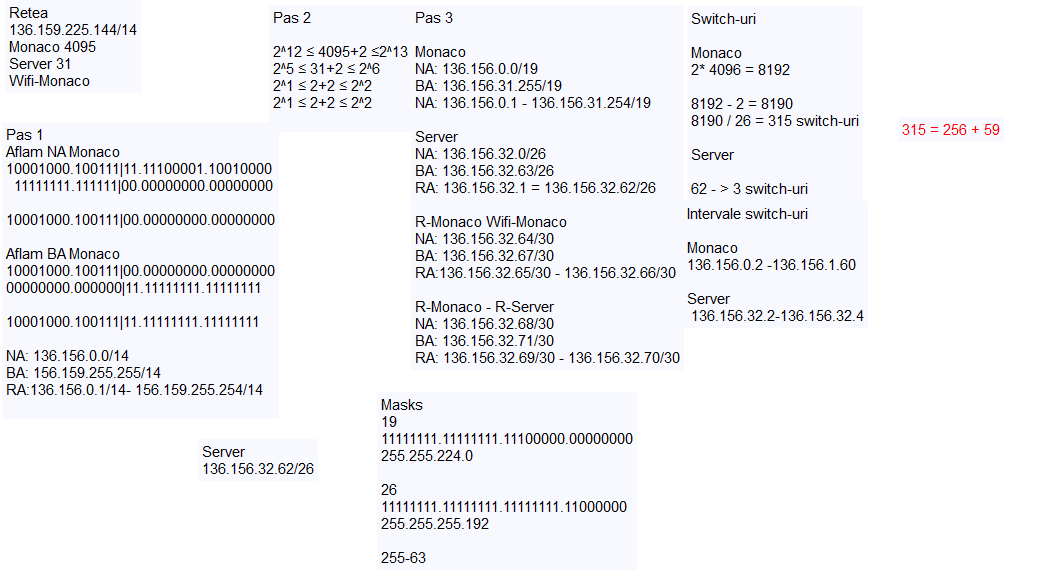
\includegraphics[width=1\linewidth]{Lab6Notite.png}
\end{center}

\newpage
\subsubsection{Cei 3 pasi}
Pentru toate 3 (si pasul 4* care nu cred ca e chiar obligatoriu dar e cam necesar si suficient de mare pentru a fi ca un pas 4)

\begin{itemize}
    \item[Pas 1] Aflarea de Network Address, Broadcast Address si Range Address pentru adresa de retea pe care o primim in input....Prin calcul binar in "tabel" cu tot cu AND-ul si OR-ul pe biti ce se vede in poza, DAR neaparat si pipe-ul $`\|` $ care reprezinta unde s-ar incheia masca cu care facem operatia pe biti.
    \item[Pas 2] Incadrarea numarului de u(seri) pentru fiecare retea LAN intre puteri de 2. Reamintim faptul ca pentru fiecare retea LAN, avem desigur IP-urile pe care le alocam echipamentelor, dar si IP-urile pentru Network Address si Broadcast Address respectiv, care NU sunt asignabile, deci trebuie sa facem mereu u+2, abia apoi incadram in puteri de 2.

    IMPORTANT. In CPT, ca sa scriem simbolul de mai mic sau egal in notite: $\leq \Leftrightarrow \&$le;
    
    \item[Pas 3] Scrierea de NA, BA, RA pentru fiecare subretea in parte.
    
    \item[Pas 4*] Calculul de intervale de switch-uri, aflata prin impartirea numarului de adrese asignabile din subretea la 26, si rotunjirea superioara. Cam este necesara ca sa dam IP-ul corect pentru primul user PC din subretea. Si sigur va fi necesara daca dorim sa configuram serviciul de DHCP.
    \item[Sfat]  La final, sa va scrieti alaturi si adresele IP pentru fiecare bucata de echipament in parte + reprezentarea mastilor, ajuta foarte mult. De exemplu adresa de server se introduce de cel putin 8 ori.
\end{itemize}


\subsection{Input}
\begin{center}
    \textbf{Input}   
    
    \begin{tabular}{|c|c|}\hline
         IP & 136.159.225.144/14 \\
         \hline \hline
         Monaco Users& 4095 \\ \hline
         Server Users& 31 \\\hline
         Wi-Fi ? & DA \\\hline
    \end{tabular}
\end{center}

\subsection{Trecand prin calcule}
\subsubsection{Pas 1}
Intai incepem prin a lucra cu adresa de retea pe care o primim, \underline{136.159.225.144/14}.

Observand ca masca este de /14, asta inseamna ca vom fixa primii 14 biti, adica primul octet in intregime si primii 6 biti din al 2-lea octet, restul vor varia.

In calcule rapide din priviri, asta ar insemna ca noi conservam octetul 136. Octetul 159 va avea afectati doar cei mai nesimnificativi 2 biti, adica valoarea va varia maxim cu 2+1=3. Iar octetii 225 si 144 vor disparea complet doar fiindca sunt 2 octeti neacoperiti de masca. 

Acum trebuie sa si demonstram asta, adica sa facem calcule. Primul pas este sa facem conversia din decimal in binar, dar pe un note.

Un \underline{sfat} pentru asta este sa incercati sa vedeti acele numere ca sume de puteri de 2 (ceea ce vor si devenii). 

Adica:
\begin{itemize}
    \item[136.]  136 = 128 + 8 
    $\rightarrow$\underline{1}000\underline{1}000

    
    \item[159.]  159 - 136 = 23 = 16 + 4 + 2 + 1 (nu avem suprapunere de puteri cu ce contine 136 deci putem adauga pur si simplu) $\rightarrow$ 100\underline{1}1\underline{111}

    sau mai intuitiv

    159 = 128 + 31

    128 = $2^{8}$ = 10000000

    31 = $2^{5} - 1$ = 00011111
    
    159 $\rightarrow$ 10011111
    
    \item[225.] 128 + 64 = 192 $\rightarrow$ \underline{11}000000

    225 - 192 = 33 = 32 + 1 $\rightarrow$ 00\underline{\underline{1}}0000\underline{\underline{1}}

    $\rightarrow$\underline{11}\underline{\underline{1}}0000\underline{\underline{1}} (calculat practic degeaba, ca nu e sub masca, dar ni se cere)

\item[144.] 144 = 128 + 16 $\rightarrow$ 10010000 (calculat practic tot degeaba, ca nu e sub masca, dar ni se cere)
\end{itemize}

Acum facem AND cu masca


\begin{center}
   \begin{tabular}{|c|c|c|}
   \hline
        Original & 136.159.225.144/14 &  IPv4 address\\
    \hline
      4 octeti &  \underline{10001000.100111}11.11000000.10010000 & adresa  \\
    \hline
      Masca &  \underline{11111111.111111}00.00000000.00000000 & primii 14 biti \\
    \hline \hline
       AND & \underline{10001000.100111}00.00000000.00000000 &  Network Address\\
    \hline
        Decimal & NA = 136.156.0.0/14 &  Network Address\\
    \hline
    \end{tabular}
\end{center}


\begin{center}
   \begin{tabular}{|c|c|c|}
   \hline

      Network Address &  10001000.100111\underline{00.00000000.00000000} & adresa  \\
    \hline
      Masca negata &  00000000.000000\underline{11.11111111.11111111} & ultimii 18 biti \\
    \hline \hline
       OR & 10001000.100111\underline{11.11111111.11111111} & Broadcast Address\\
    \hline
        Decimal & 136.159.255.255/14 &  Broadcast Address\\
    \hline
    \end{tabular}
\end{center}

Deci avem pentru reteaua principala, adica cea mare ce le va contine pe toate:

NA = 36.156.0.0/14

BA = 136.159.255.255/14

RA = 36.156.0.1/14 - 136.159.255.254/14

\subsubsection{Pas 2}
Cate subretele avem ? 4. (Patru), IV, FOUR, U+56DB.
\begin{itemize}
    \item LAN Monaco (Subreteaua principala)
    \item LAN Server (Subreteaua dedicata Server)
    \item R-Monaco - R-Server (Subreteaua de legatura cu server)
    \item R-Monaco - Wi-FiMonaco (Subreteaua de legatura cu Router-ul de Wi-Fi)

    
    \item LAN Wi-Fi de care se ocupa wi-fi router-ul intr-un fel. Mai mult decat noi. Dar totodata va face parte din Monaco. (e o minciuna si el)
\end{itemize}

\paragraph{Monaco}
Reteaua Monaco, va avea 4095 users, si desi pare ca 4095$\leq$ 4096 = $2^{12}$, si asta este o minciuna!

Nu uitati ca mereu adaugam +2, deoarece NA+BA nu sunt asignabile, deci nu se includ in alea 4095.

Iar 2+4095 = 4097 $>$ 4096

Asadar mergem la urmatoarea putere de 2 ca upper-bound, $2^{13}$. Si masca va fi de 32-13 = 19 bits. O masca de 19 biti sau 255.255.224.0

\[2^{12} \leq 4095+2 \leq 2^{13}\]

Deci noi de fapt vom avea 2*4096 = 8192 de adrese dintre care 8190 asignabile.

Si deoarece LaTeX-ul din CPT este putin mai ciudat decat cel din overleaf, nu uitati ca in note veti scrie practic 

\begin{verbatim}
                    2^12 &le; 4095+2 &le; 2^13
\end{verbatim}

\paragraph{Server}
Aceeasi teorie.

31 + 2 = 33 $>32 = 2^5$ 

Deci vom creste iar masca.

\[2^{5} \leq 31+2 \leq 2^{6}\]

Asadar o masca de 32-6 = 26 bits, sau o masca de 255.255.255.192.0

Vom avea 64 de adrese totale, dintre care 64-2=62 ip-uri asignabile.

\paragraph{R-Monaco - R-Server}

O subretea mai interesanta in sensul ca aceasta leaga cele 2 subretele de mai sus, si in acelasi timp formeaza propria sub-retea. Este formata doar din 2 routere si atat. (nu e nevoie de switch-uri, si default-gateway putem seta ca oricare dintre cele 2 routere, ca oricum asta este rolul lor)

Deci vom avea 2 adrese de ip asignabile, +2 de NA si BA.

\[2^{1} \leq 2+2 \leq 2^{2}\]


\paragraph{R-Monaco - Wi-FiMonaco}

Aceeasi idee de mai sus, deaorece Router-ul de Wifi este si el tot un fel de router, deci ii putem lega LAN-ul de Wi-Fi cu LAN-ul de Monaco.



\[2^{1} \leq 2+2 \leq 2^{2}\]


\subsubsection{Pas 3}
\paragraph{Monaco}

Sortam descrescator LAN-urile dupa numarul de utilizatori. Prima este Monaco.

Incepem de la adresa de retea, 136.156.0.0, ignoram masca.

Adaugam masca de Monaco. 32-13 = /19

NA = 136.156.0.0/19

Aflam BA



\begin{center}
   \begin{tabular}{|c|c|c|}
   \hline

      Network Address &  10001000.10011100.000\underline{00000.00000000} & adresa  \\
    \hline
      Masca negata &  00000000.00000000.000\underline{11111.11111111} & ultimii 13 biti \\
    \hline \hline
       OR & 10001000.10011100.000\underline{11111.11111111} & Broadcast Address\\
    \hline
        Decimal & 136.156.31.255/19 &  Broadcast Address\\
    \hline
    \end{tabular}
\end{center}

NA = 136.156.0.0/19

BA = 136.156.31.255/19

RA = 136.156.0.1/19 136.156.31.254/19


\paragraph{Server}

Incepem de la adresa de Broadcast de la Monaco +1 , 136.156.32.0, ignoram masca.

Adaugam masca de Server. 32-6 = /26

NA = 136.156.32.0/26

Aflam BA
\begin{center}
   \begin{tabular}{|c|c|c|}
   \hline

      Network Address &  10001000.10011100.00100000.00\underline{000000} & adresa  \\
    \hline
      Masca negata &  00000000.00000000.00000000.00\underline{111111} & ultimii 6 biti \\
    \hline \hline
       OR & 10001000.10011100.00100000.00\underline{111111} & Broadcast Address\\
    \hline
        Decimal & 136.156.32.63/26 &  Broadcast Address\\
    \hline
    \end{tabular}
\end{center}

NA = 136.156.32.0/26

BA = 136.156.32.63/26

RA = 136.156.32.1/26 - 136.156.32.62/26

\newpage
\paragraph{Legaturile}

Practic aici avem doar 4 adrese in toata subreteaua deci nici nu mai ar fi ce tabel sa facem, ci doar o adunare de +1/+2/+3/+4 cu BA-ul de Server. De mentionat ca legaturile se fac in ordinea in care primim retelele. ("Din aproape in aproape")


\begin{center}

    R-Monaco - Wi-FiMonaco


    \begin{tabular}{|c|c|} \hline
         NA & 136.156.32.64/30 \\ \hline
         BA & 136.156.32.67/30\\ \hline
         RA & 136.156.32.65/30 - 136.156.32.66/30 \\ \hline
    \end{tabular}
    


    R-Monaco - R-Server

    \begin{tabular}{|c|c|} \hline
         NA & 136.156.32.68/30 \\ \hline
         BA & 136.156.32.71/30\\ \hline
         RA & 136.156.32.69/30 - 136.156.32.70/30 \\ \hline
    \end{tabular}

\end{center}

\subsubsection{Pas4*}

Pentru Monaco si Wi-Fi ne va interesa sa punem si switch-uri, dar cate si unde?

1. Impartim numarul de adrese asignabile la 26.

2. Adaugam la DGW.


\paragraph{Monaco} 8190 ip-uri.

\[\frac{8190}{26} = 315\]

dar \[315 = 256 + 59\]

First Switch = NA+1+1 = 136.156.0.1 + 1 = 136.156.0.2/19

Last Switch = NA+1+315 = 136.156.0.1 + 256 + 59 = 136.156.1.60/19



\textbf{Switch Range} 
\[36.156.0.2/19 - 36.156.1.60/19\]

Primul user Host = 136.156.1.61/19

\paragraph{Server} 62 ip-uri

\[ \frac{62}{26}=2,384615384615385 \approx3\]

First Switch = NA+1+1 = 136.156.32.1/26 + 1 = 136.156.32.2/26

Last Switch = NA+1+3 = 136.156.32.1/26 + 3 = 136.156.32.4/26


\textbf{Switch Range} 
\[136.156.0.2/26 - 136.156.1.4/26\]


Primul user Host = 136.156.32.5/26

(Fiind o subretea dedicata pentru server nu prea e cazul sa si punem acel pc-host).

\subsubsection{Also.}
Also mai ar fi o recomandare sa va notati numeroasele adrese si masti..eg

Ce am pus eu in "Adrese for me"

Masti


/19 = 255.255.224.0

/26 = 255.255.255.192

Monaco PC = 136.156.1.61/19

Monaco Switch = 136.156.0.2/19

Monaco Router = 136.156.0.1/19


Server = 136.156.32.62/26

R-Server = 136.156.32.1/26

\subsubsection{DHCP}

Mai adaugam un pc legat de SwMonaco, ii vom atribui adresa dinamic prin serviciul de DHCP. pentru asta ne folosim de switch range-ul calculat mai devreme. Configurarea este chiar scurta.

Helper-address-ul va fi adresa de unde R-Monaco va primi adresele de IP prin DHCP, adica adresa de pe portul serial0/0/0 a lui R-Server, pe care o configuram pe portul gigabit0/0, deoarece pe acest port R-Monaco actioneaza ca DefaultGateway.

De ce excluded-address este "136.156.0.1 136.156.1.61"?

Deoarece aceasta este intervalul de DGW + switch-uri + pc-ul configurat static de noi mai devreme.







\begin{verbatim}
R-Monaco(config)#interface giga0/0
R-Monaco(config)#ip helper-address 136.156.32.70
R-Monaco(config)#exit

.....

R-Server(config)#ip dhcp excluded-address 136.156.0.1 136.156.1.61
R-Server(config)#ip dhcp pool Monaco
R-Server(dhcp-config)#network 136.156.0.0 255.255.224.0
R-Server(dhcp-config)#default-router 136.156.0.1
R-Server(dhcp-config)#dns-server 136.156.32.62
\end{verbatim}

End Devices $\rightarrow$ End Devices $\rightarrow$ PC $\rightarrow$ Schimbam portul si legam de switch.



Click $\rightarrow$ Desktop $\rightarrow$ IP Config $\rightarrow$ DHCP





\subsubsection{Concluzie}

\begin{center}
    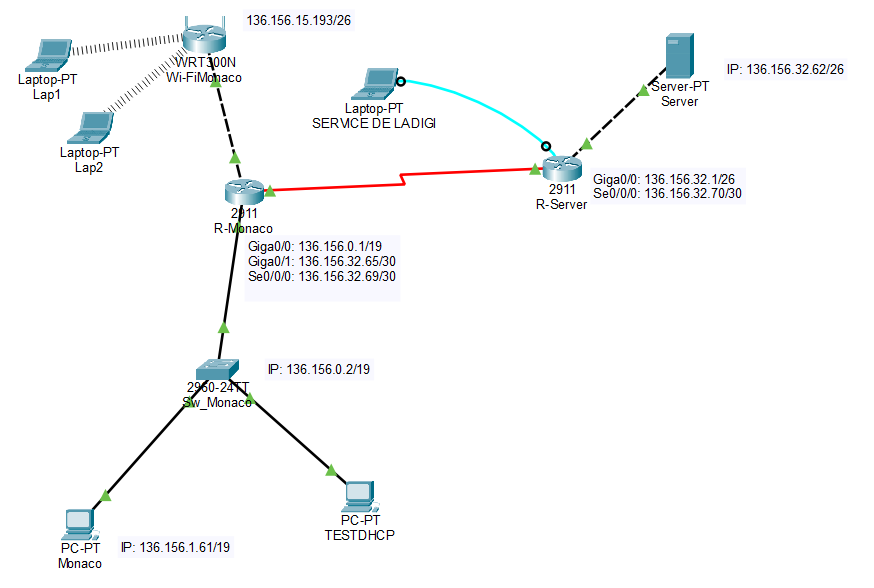
\includegraphics[width=1\linewidth]{PozaLab6.png}
\end{center}


\section{Lab7 Test2}
Un exemplu a ce puteti sa primiti la examen.
\begin{center}

    Inputs:
    
    \begin{tabular}{|c|c|}\hline
        IP: & 201.240.168.210/16 \\\hline
         Tismana 1& 1023 \\ \hline
         Tismana 2& 31\\ \hline
         Tismana 3& 2046 \\ \hline
         Tismana 4& 4095\\ \hline
         Wi-Fi Tismana2? & Da \\ \hline
         Server Tismana1? & Da \\\hline
    \end{tabular}
\end{center}

\begin{center}
    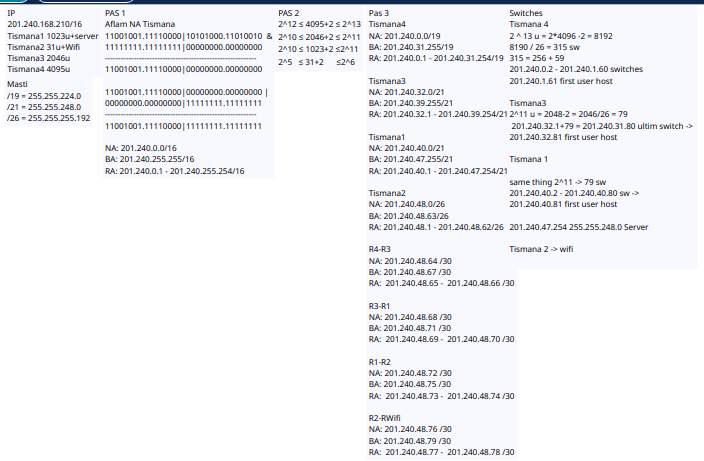
\includegraphics[width=1\linewidth]{NotiteLab7.png}
\end{center}
\part{Optional MAC An III}

\part{Q.E.D.}

$\rightarrow$

$\leq$




\begin{center}
    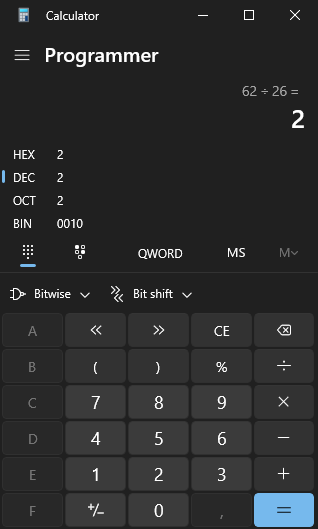
\includegraphics[width=0.5\linewidth]{wtf.png}
    
    Imagineaza-ti sa vezi asta la 1 dimineata
\end{center}



Btw am atins aproape jumatate de MB in fisier... damn.

\end{document}
